\documentclass[10pt, openany]{book}
\usepackage{header}
\pgfplotsset{compat=1.18}
\AtBeginDocument{\RenewCommandCopy\qty\SI}

\title{EE Notes}
\author{Damanic Luck}
\date{April 14, 2024}

\begin{document}
% Use this website to find symbols: https://detexify.kirelabs.org/classify.html

\maketitle
% \setcounter{chapter}{1}

\tableofcontents
\begin{todo}
    \item use this article \href{http://home.iitj.ac.in/~sptiwari/EE314/Lecture2_Semi_Basics_Junction.pdf}{to add to ch1 about doping}
    \item practice problems for ch1
    \item practice problems for ch2
    \item practice problems for ch3
    \item finish up ch3 i burned out while trying to be thorough. p117 in reader, p152 in sedra
    \item go through ch1-5 to change any units instead with the \SI{5}{\kilo \ohm} etc command OR THE \unit[per-mode=symbol]{\kilo \ohm}
\end{todo}

% CHARGE CARRIERS AND DOPING
\newpage
\section{Charge Carriers and Doping}

\subsection{Introduction}
We start learning about resistors, capacitors, and inductors from earlier courses such as EECS 16A and 16B. With more components like transistors, diodes, and op-amps (which are all based on semiconductors), we are able to expand upon circuit design. We need to understand semiconductor physics in order to understand how these components operate.
\begin{center}
    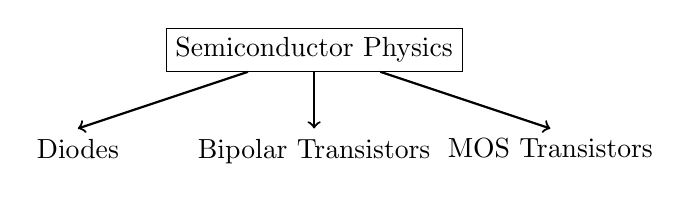
\begin{tikzpicture}
        \node[draw, align=center] (text) {Semiconductor Physics};
        \draw[->, thick] (text) -- ++(0,-1) node[below] {Bipolar Transistors};
        \draw[->, thick] (text) -- ++(-3,-1) node[below] {Diodes};
        \draw[->, thick] (text) -- ++(3,-1) node[below] {MOS Transistors};
    \end{tikzpicture}
\end{center}

We can also redefine Ohm's Law which we know as ($V = IR$) as $J = \sigma \vb{E}$. We can also write resistance($R$) and conductance($G$) in terms of other variables
\begin{gline}
    \item $J$: current density, $A/m^2$ (Amperes per meter squared)
    \item $\sigma$: conductivity, $S/m$ (Siemens per meter)
    \item $\vb{E}$: electric field, $V/m$ (Volts per meter)
\end{gline}

$R = \frac{R}{I} = \rho \frac{l}{A}$ and $G = R^{-1} = \sigma \frac{A}{l}$
\begin{gline}
    \item $\sigma$: conductivity
    \item $\rho$: resistivity
\end{gline}

For collisions in gas, we focus on the idea that initial velocity and direction is lost/randomized after a few collisions. So, when we sum over the random velocities of the particles and average it, it comes out to zero. Average momentum gain is:
\[\bar{\mu} = \frac{\vb{E} q \tau}{M} = \mu \vb{E}, ~~~ \mu := \frac{q \tau}{M} = \frac{\bar{v}}{\vb{E}}\]
\begin{gline}
    \item $\mu$: mobility, $m^2/ (V \cdot s)$
    \item $q$: electric charge, $1.60 \times 10^{-19}$, Coulombs = Amperes/second
    \item $\tau$: mean free time
    \item $M$: mass
    \item $\bar{v}$: average velocity
\end{gline}

Different elements have a different number of outer shell electrons. For semiconductors like silicon, we can increase the temperature to increase its conductivity. Silicon atoms are arranged in a diamond structure and in general, the energy levels that an atom can occupy are discrete. The \textbf{valence band} electrons are at a lower energy state (bound to host atoms) while \textbf{conduction band} electrons are at a higher energy state and are "free" electrons. These electrons are free to move around the crystal and take part in conduction. 

\subsection{Conduction and Fermi Dirac Distribution}
Thermal energy is on average about $\sim 26~eV$ at room temperature How large the \textbf{band-gap}, the gap between the conduction and valence band, determines how conductive a material is:
\begin{itemize}
    \item Insulators: band gap $\sim$ 15 $eV$
    \begin{itemize}
        \item Glass, rubber, oil, plastic, diamond
    \end{itemize}
    \item Semiconductors: band gap $\sim 1 eV$
    \begin{itemize}
        \item Silicon = 1.12 $eV$
    \end{itemize}
    \item Conductors: Not applicable due to overlapping conduction/valence bands
\end{itemize}
Because electrons are a type of particle called a \textbf{fermion}, we can say that 
\[f(\epsilon) = \frac{1}{e^{\frac{E - E_F}{k_B T}} + 1}\]
\begin{gline}
    \item $f(\epsilon)$: occupational probability of a state energy $\epsilon$
    \item $E_F$: fermi energy, $eV$
    \item $k_B$: Boltzmann's constant, $1.380649 \times 10^{-23} J/K$ (Joules per Kelvin)
    \item $T$: temperature in Kelvin
\end{gline}
\subsection{Doping}
\textbf{Doping} is defined as introducing impurities inside a silicon crystal to adjust the number of free electrons that we have. The following materials are commonly used:
\begin{pline}
    \item Group III elements: boron, aluminum, gallium $\rightarrow$ acceptors
    \item Group IV elements: germanium and silicon
    \item Group V elements: phosphorus, arsenic, antimony $\rightarrow$ donors
\end{pline}
Sometimes we assume that the number of electrons we add is much greater than the original free electrons that pure silicon had ($10^{10}$ per cubic centimeter). This leads to the simplification that the number of free electrons in our silicon crystal is $N_D$, where $N_D$ is the number of donor atoms that we add per cubic centimeter.

\subsection{Practice Problems}

\subsection{Sources}
\begin{itemize}
    \item \href{https://www.youtube.com/watch?v=yQDfVJzEymI}{\textcolor{blue}{Razavi Electronics 1, Lec 1, Intro., Charge Carriers, Doping}}
    \item \href{https://file.notion.so/f/f/048d6522-202b-48d4-b5d9-bc005bd602e2/214bf1f0-292f-48d6-9016-737d9f5da155/ee105_reader_v3.pdf?id=237a4300-3dbe-47d1-888b-ffae90d8352b&table=block&spaceId=048d6522-202b-48d4-b5d9-bc005bd602e2&expirationTimestamp=1714435200000&signature=yx-H1qvZJIodPfazOpwXX0Ce2mWMG8skOHl45xoPxus&downloadName=ee105_reader_v3.pdf}{EE105 Reader}
    \item Sedra, Adel S., et al. Microelectronic Circuits. Oxford University Press, 2021
    \item \href{https://eng.libretexts.org/Bookshelves/Materials_Science/TLP_Library_II/22%3A_Introduction_to_Semiconductors/22.2%3A_The_FermiDirac_Distribution}{Engineering LibreTexts: The Fermi-Dirac Distribution}
\end{itemize}



% DRIFT AND DIFFUSION CURRENT
\newpage
\section{Doping and Drift}

\subsection{Sources}
\begin{itemize}
    \item \href{https://www.youtube.com/watch?v=NWolpDgi6_Y}{\textcolor{blue}{Razavi Electronics 1, Lec 2. Doping, Drift}}
\end{itemize}

% PN JUNCTIONS
\newpage
\chapter{PN Junctions}

A \textbf{PN junction} is the junction between an $N$-type semiconductor and $P$-type semiconductor. Understanding the PN junction will set up us for understanding diodes, BJTs, and MOSFETs later. It seems like we draw it as two separate silicon crystals, but in actual practice the $p$ and $n$ regions are part of the same silicon crystal, accomplished by creating regions of different doping.

Plus ("+") signs represent majority holes while minus ("-") signs represent majority el ectrons. The following diagram is from Seda and Adel's \textit{Microelectronic Circuits}.

\begin{figure}[htb]
    \centering
    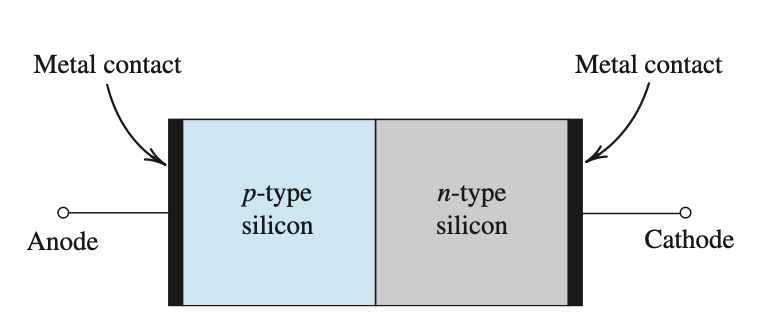
\includegraphics{figs/ch03/pn_junction.png}
    \caption{Simplified physical structure of the PN junction}
\end{figure}

\section{Diffusion Current}
Although it doesn't show it in the diagram, there minority holes generated by thermal ionization in the $n$-type material and there are minority electrons generated in the $p$-type material. Due to concentration difference of holes in the $p$ region and the $n$ region, holes diffuse across the junction from the $p$ side to the $n$ side. This results in \textbf{diffusion current, $I_D$}, whose direction is from the $p$ to $n$ side.

So current Damanic is wondering right now "if this stuff is diffusing then won't this entire block be the same mush at the end." Here we introduce the depletion region. Holes that diffuse across the junction into the $n$ region recombine with majority electrons there. A charge is said to be \textbf{uncovered} when some of the bound positive charge is no longer neutralized by free electrons. This introduces the idea that at a region close to the junction, it is depleted of free electrons and contains unbound positive charge for the $n$ region.

\begin{figure}[htb]
    \centering
    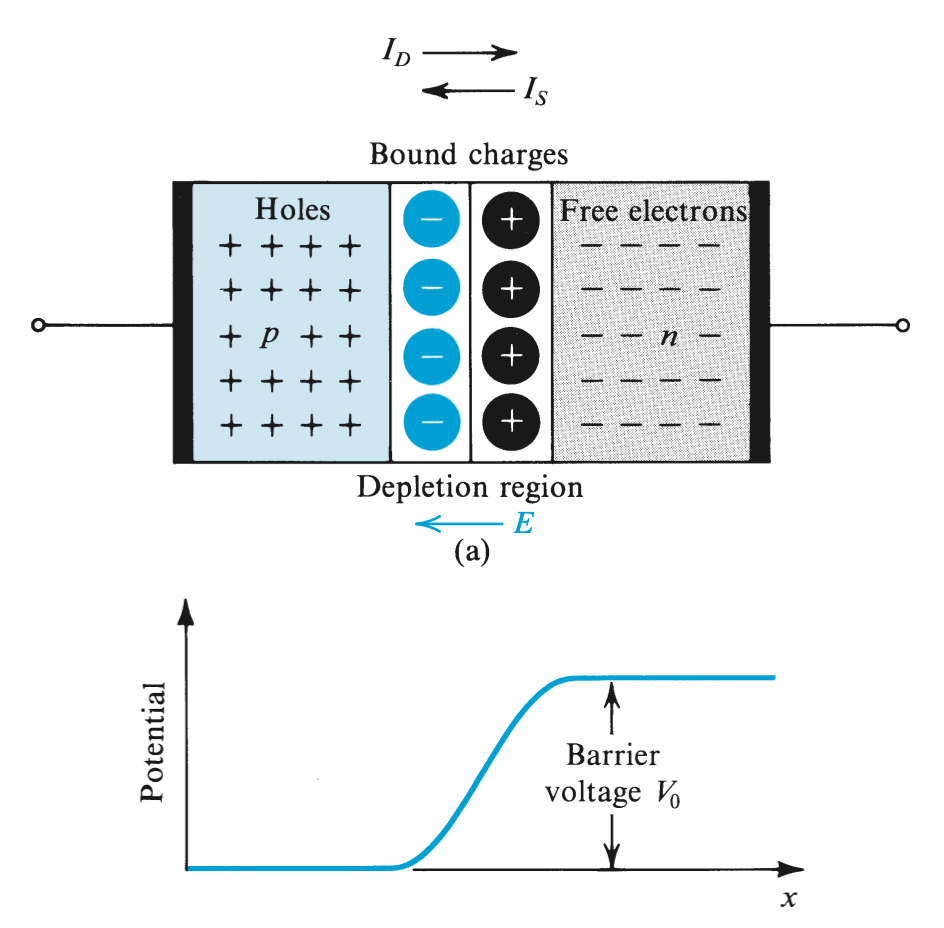
\includegraphics[scale=0.5]{figs/ch03/uncovered_region.png}
    \caption{Top image shows PN-junction with bound charges and bottom image is potential along an axis perpendicular to the junction}
    \label{fig:barrier-voltage1}
\end{figure}

The left side of the PN junction ($p$ region) will be negatively charged while the right side ($n$ region) will be positively charged. To sum it up, this is because at some point, electrons that diffuse across the junction into the $p$ region will recombine with holes, and those holes will disappear leaving uncovered bound negative charge. Vice versa for holes diffusing into the $n$ region. 

From the figure above we see that the $n$ region will be positively charged and the $p$ side if negatively charged. This is the \textbf{depletion region}, or the \textbf{space-charge region} or \textbf{depletion layer}. There are no \textit{mobile} charge carriers present here. Charges on both sides of the depletion region results in an electric field $E$. Here we introduce the idea that a larger barrier voltage results in a small number of carriers that can overcome this barrier. This leads to a decrease in magnitude of diffusion current since it is more difficult for holes to diffuse into the $n$ region and electrons to diffuse into the $p$ region. Referring again to figure \ref{fig:barrier-voltage1}, we see that $V_0$ is the barrier voltage. Therefore the diffusion current $I_D$ has a strong relationship with $V_0$, the voltage drop across the depletion region.

\section{Drift Current and Equilibrium}
Recall that drift current is caused by electric fields and $I_S$ is independent of the value of the depletion-layer voltage $V_0$. Under open-circuit conditions, there is no external current, so 
    \[I_D = I_S\]
This condition is maintained by $V_0$.
\begin{Analysis}{$I_S$ and $I_D$ at Equilibrium}{}
    \begin{gline}
        \item $V_O$: barrier voltage
        \item $I_S$: drift current whose direction is from the $n$ side to the $p$ side of the junction
        \item $I_D$: diffusion current whose direction is from the $p$ side to the $n$ side of the junction
    \end{gline}
    \begin{enumerate}
        \item \textbf{$I_D > I_S$}: more bound charge is uncovered on both sides $\rightarrow$ the depletion layer widens (vertically)$\rightarrow$ $V_0$ increases $\rightarrow$ $I_D$ decreases until $I_D = I_S$ (equilibrium)
        \item \textbf{$I_D < I_S$}: uncovered charge decreases $\rightarrow$ depletion layer narrows (vertically) $\rightarrow$ $V_0$ decreases $\rightarrow$ $I_D$ increases until $I_D = I_S$ (equilibrium)
    \end{enumerate}
\end{Analysis}

Under the zero bias equilibrium condition (no external voltage is applied to the PN junction), does the diffusion and drift current "cancel" out here, meaning that current density is nearly zero. Their individual components are also equal here, i.e. hole/electron drift current is equal to hole/electron diffusion current, respectively.

    \[J_n = 0 = qn_0 \mu_n E_0 + q D_n \frac{dn_0}{dx}\]

$V_0$ has been referred to so far as barrier voltage boltage, but it's also called \textbf{junction built-in voltage}.
    \[\phi_{bi} = V_{th} \ln \left(\frac{N_A N_D}{n_i^2}\right) = \frac{kT}{q} \ln \left(\frac{N_A N_D}{n_i^2}\right)\]
Remember here that $V_th$ is thermal voltage which is $\approx$ 26 mV at room temperature. $\phi_{bi}$ is typically 0.6 V to 0.9V for room temperature silicon. In the EE105 reader, $\phi_{bi}$ and $V_{th}$ has the same meaning as $V_0$ and $V_T$, respectively, in the \textit{Microelectronic Circuits} textbook. I'm writing down the EE105 reader notation here for clarity.

\begin{figure}[htb]
    \centering
    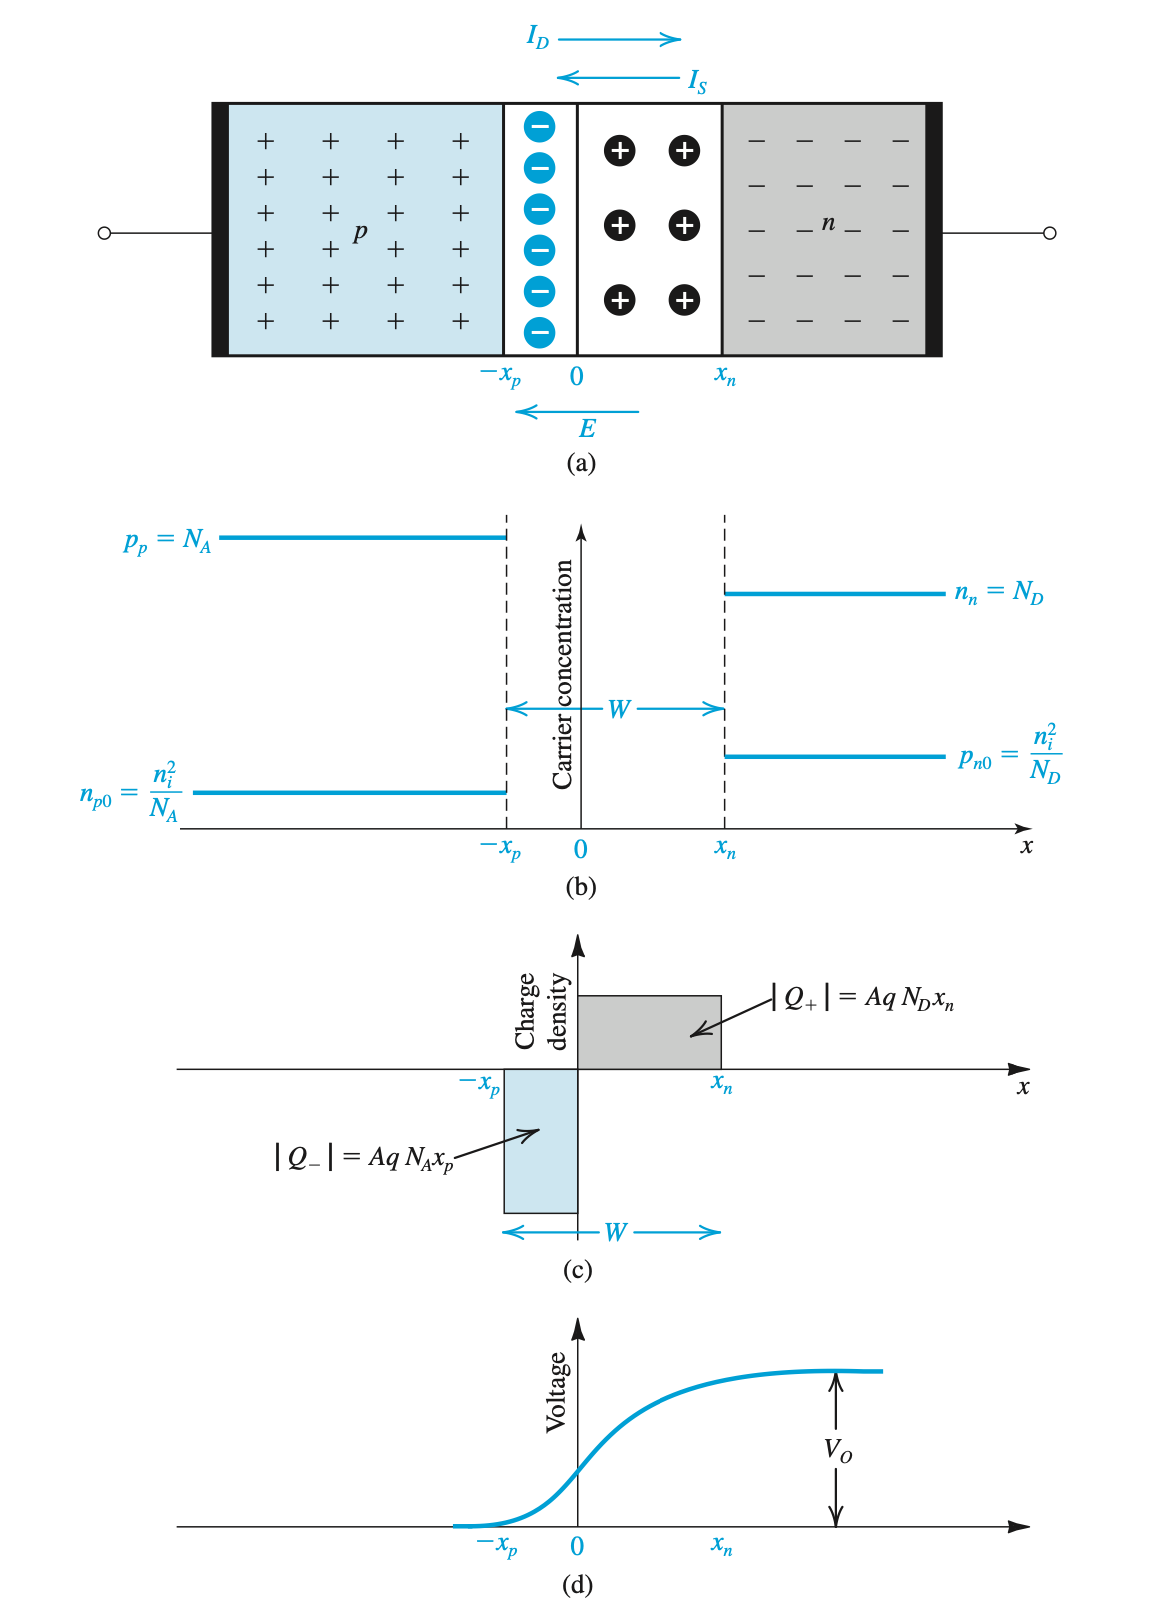
\includegraphics[scale=0.6]{figs/ch03/3_graph.png}
    \caption{Graphs of (a) a PN junction (b) carrier concentrations (c) charge density (d) built in voltage $V_0$}
    \label{fig:3figs}
\end{figure}
\begin{todo}
    \item How we got from each graph
\end{todo}
This graph shows a junction where $N_A > N_D$. If we heavily dope one side, the depletion region will exist almost entirely on the lightly doped side.

\begin{figure}[htb]
    \centering
    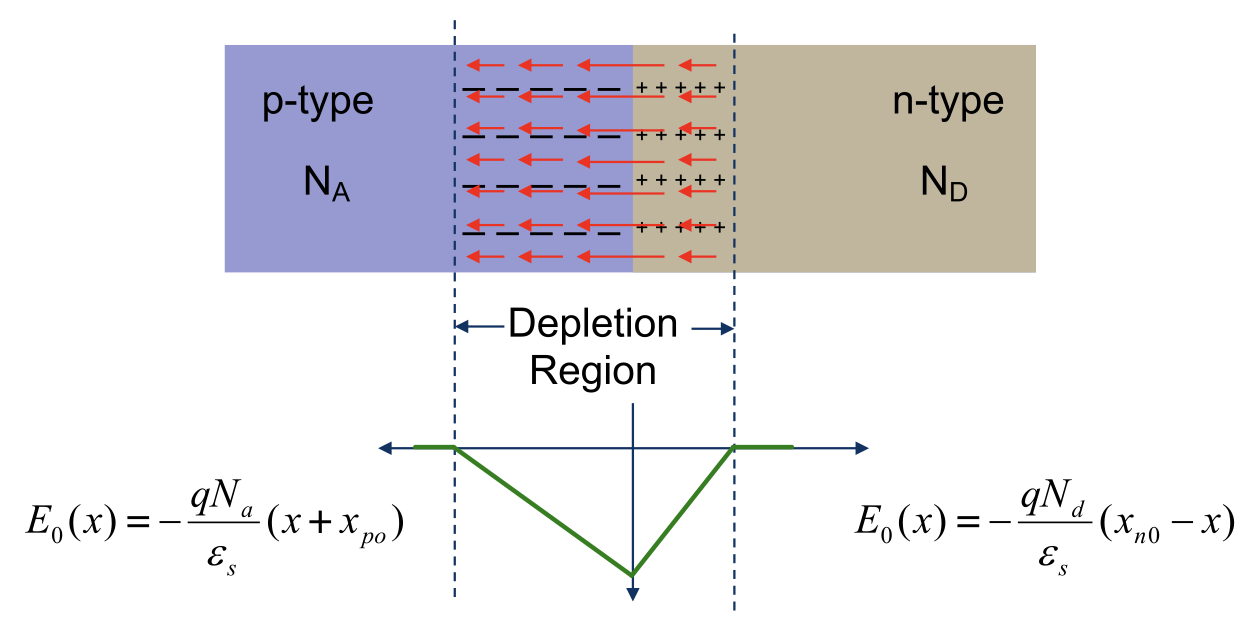
\includegraphics[scale=0.5]{figs/ch03/concentration_reader.png}
    \caption{Graph of electric field of PN junction}
    \label{fig:electric_fields_pn}
\end{figure}

Here in figure \ref{fig:electric_fields_pn}, the electric fields in the depletion region are negative because positive charges are on the right and the negative charges are on the left, assuming zero fields in neutral $P$-region and $N$-regions. Key takeaways due to difference in doping levels in the $N$-type and $P$-type sides:
\begin{pline}
    \item Width of the depletion region is not symmetric
    \item Slope of the electric field is larger in one region than the other
    \item The negative peak of the electric field always occurs at the junction
\end{pline}

\begin{Analysis}{Gauss's Law}{}
    Gauss's Law states that the total electric flux out of a closed surface is equal to the charge enclosed by the permittivity. Electric flux is the electric field multiplied by the area of the surface projected in a plane and perpendicular to the field.
        \[\oint_S {\vec{E_n} \cdot \vec{d}s = \frac{1}{{\varepsilon _0 }}} Q_{inside}\]
    \begin{todo}
        \item finish this
    \end{todo}
    By Gauss's Law, the total fixed charged in the $N$-region is the same as the total fixed charge in the $P$-region.
        \[q N_A x_{p0} = q N_D x_{n0}\]
\end{Analysis}
Here we'll derive the equations for depletion width, which are dependent on externally applied voltage, which are given by the following. The zero is for the zero bias case.
\begin{itemize}
   \item[] Depletion width on N-side: {\Large $x_{n_0} = \sqrt{\frac{2 \epsilon_s \phi_{bi}}{q N_D} (\frac{N_A}{N_A + N_D})}$}
   \item[] Depletion width on P-side: {\Large $x_{p_0} = \sqrt{\frac{2 \epsilon_s \phi_{bi}}{q N_A} (\frac{N_D}{N_A + N_D})}$}
   \item[] Built in potential: {\Large $\phi_{bi} \equiv \phi_n = \phi_p > 0$}
   \item[] Total depletion width {\Large $X_{dep_0} = x_{n_0} + x_{p_0} = \sqrt{\frac{2 \epsilon_s \phi_{bi}}{q}(\frac{1}{N_A} + \frac{1}{N_D})}$}
\end{itemize}

\begin{todo}
    \item derivation here
\end{todo}
For the zero bias case (under thermal equilibrium), net current is zero. Diffusion current is very small since few carriers have enough energy to penetrate the barrier. Drift current is small since minority carriers are few.
\section{Reverse Bias}
\begin{figure}[H]
    \centering
    \begin{circuitikz}
        \draw (0,0) to [battery2, l=$V_D < 0$ , invert] (0,2)
        to [short] (2,2)
        to [full diode, v^=$-\phi_{bi}+V_D$,] (2,0)
        to (0,0);
    \end{circuitikz}
    \label{fig:reverse_bias}
\end{figure}

The above section was discussing the PN junction at equilibrium. At equilibrium, the $PN$-junction doesn't draw any current. Under reverse bias like in figure above, meaning that a negative voltage is applied, charge will increase and the depletion region widens horizontally. We can rewrite the depletion width formulas from above as a function of $V_D$.
\begin{itemize}
    \item[] {\Large $x_n(V_D) = \sqrt{\frac{2 \epsilon_s (\phi_{bi} - V_D)}{q N_D} (\frac{N_A}{N_A + N_D})} = x_{n_0} \sqrt{1 - \frac{V_D}{\phi_{bi}}}$}
    
    \item[] {\Large $x_p(V_D) = \sqrt{\frac{2 \epsilon_s (\phi_{bi} - V_D)}{q N_A} (\frac{N_D}{N_A + N_D})} = x_{p_0} \sqrt{1 - \frac{V_D}{\phi_{bi}}}$}

    \item[] {\Large $X_{dep_0} = x_n(V_D) + x_n(V_D) = \sqrt{\frac{2 \epsilon_s (\phi_{bi} - V_D)}{q}(\frac{1}{N_A} + \frac{1}{N_D})} = X_{dep_0} \sqrt{1 - \frac{V_D}{\phi_{bi}}}$}
\end{itemize}
Keep these in mind: 
\begin{pline}
    \item Minority drift current is independent of the barrier height ($\phi_{bi}$)
    \item Diffusion current is a strong exponential function of the barrier height
\end{pline}

\section{Forward Bias}
This occurs when $V_D$ is nonnegative. A forward bias results in a exponential increase in the number of carriers, which have enough energy to break the barrier. This results in an exponential increase in diffusion current. Drift current doesn't change with forward bias. 

\begin{todo}
    \item skipped small signal model for this
    \item skipped a lot of practice problems for this too
\end{todo}

\section{Practice Problems}
\begin{enumerate}
    \item Show that 
        \[V_0 = \frac12 (\frac{q}{\epsilon_s})(\frac{N_A N_D}{N_A + N_D}) W^2\]
    % \begin{Ans}
    %     We know that $\phi_{bi} = V_{th} \ln \left(\frac{N_A N_D}{n_i^2}\right) = \frac{kT}{q} \ln \left(\frac{N_A N_D}{n_i^2}\right)$
    % \end{Ans}
    \item Show that for a PN junction in which the $p$ side is much more heavily dped than the $n$ side (i.e. $N_A \gg N_D$) referred to as a $p^+ n$ diode. The following can be written as follows:
        \begin{align*}
            W &\simeq \sqrt{\frac{2 \epsilon_s}{q N_D}V_0}, ~~~~~ x_n \simeq W, ~~~~~ x_p \simeq \frac{W}{N_A / N_D} \\
            Q_j &\simeq A q N_D W, ~~~~~ Q_j \simeq A \sqrt{2 \epsilon_s q N_D V_0}
        \end{align*}
    
    \item For a Si PN junction that looks like this, where $N_A = 1 \times 10^{18}$ \conc and $N_D = 1 \times 10^{17}$ \conc. Given the built-in potential is 0. V and the relatively permittivity of Si is 12. No voltage is applied.
    \begin{figure}[H]
        \centering
        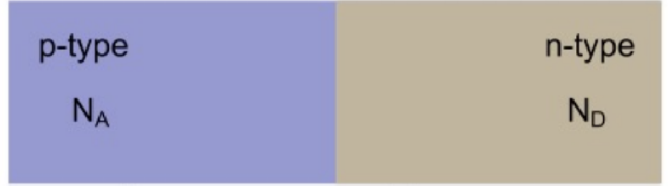
\includegraphics[scale=0.5]{figs/ch03/ans2.png}
    \end{figure}
    \begin{enumerate}
        \item Draw the charge along the horizontal axis.
        \item Draw the electric field along the horizontal axis. Label the critical points such as charge density, depletion width, and maximum electric field in your graphs.
    \end{enumerate}

    \item Considering a PN junction where the $n$ side is doped with $N_D = 10^{17}$ \conc and $p$ side is doped with $N_A = 10^{20}$ \conc, $n_i = 10^{10}$ \conc, kT/q = 26 mV, $\mu$n = 100 \mobility at $p$ side, $\mu$p = 400 \mobility at n side, L$_n$ = 2.3 \mun at $p$ side, and L$_p$ = 3.2 \mun at $n$ side, vacumn permittivity is $\epsilon_0 = 8.854 \times 10^{-12}$ C\sq/ (N $\cdot$ m\sq), the permittivity of silicon is 11.7$\epsilon_0$. Area of the PN junction is 1 \mun\sq
    \begin{enumerate}
        \item Calculate the built-in potential.
        \item Calculate the total depletion width at zero bias.
        \item Draw the electric field profile at zero bias (You need to calculate the maximum electric field). The left-hand side is N and the right-hand side is P.
        \item Calculate the depletion capacitance when the bias -1V. 
        \item Calculate the current when the bias is 1V.
        \item Find out the small-signal resistance and diffusion capacitance at 1V Given $\tau = 1 \mu$s. 
    \end{enumerate}
\end{enumerate}

\section{Sources}
\begin{itemize}
    \item Sedra, Adel S., et al. Microelectronic Circuits. Oxford University Press, 2021: Specifically screenshots of the graphs I need to redo this when I learn how to use graphing/tikzpicture better in LaTex
    \item \href{https://file.notion.so/f/f/048d6522-202b-48d4-b5d9-bc005bd602e2/214bf1f0-292f-48d6-9016-737d9f5da155/ee105_reader_v3.pdf?id=237a4300-3dbe-47d1-888b-ffae90d8352b&table=block&spaceId=048d6522-202b-48d4-b5d9-bc005bd602e2&expirationTimestamp=1714435200000&signature=yx-H1qvZJIodPfazOpwXX0Ce2mWMG8skOHl45xoPxus&downloadName=ee105_reader_v3.pdf}{EE105 Reader}
    \item Q1 and Q2 are excercises from Sedra, Adel chapter3
    \item Q3 from here is Q4 from EE105 HW6
    \item Q4 from here is Q1 from EE105 Hw7
    \item \href{https://byjus.com/jee/gauss-law/}{Explanation of Gauss's Law}
\end{itemize}

% MOSCAP
\newpage
\chapter{MOS Capacitor}
The MOS in MOS capacitor stands for Metal-Oxide-Silicon. Sometimes the S is also written as substrate in other places. Understanding threshold voltage here for a MOS-CAP is useful for also understanding MOSFETs in a later chapter.
\begin{pline}
    \item Metal: usually this ia  heavily doped polysilicon (Poly-$Si$) layer doped with $n^+$ or $p^+$, due to high temperature processing for aluminum
    \item Oxide: SiO$_2$ where $\epsilon_{ox} = 3.9 \epsilon_0$, can be any insulator actually
    \item Substrate: $\epsilon_s = 11.7 \epsilon_0$; NMOS capacitor $\rightarrow$ $P$-type substrate, PMOS capacitor $\rightarrow$ $N$-type substrate
\end{pline}

\section{MOSCAP at Equilibrium}
\begin{figure}[H]
    \centering
    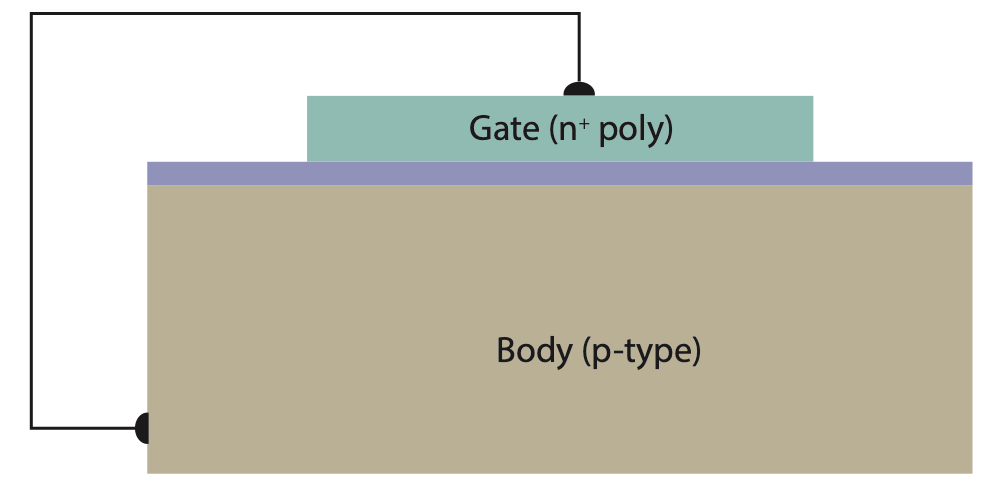
\includegraphics[scale=0.4]{figs/ch04/moscap_short.png}
    \caption{MOS CAP with gate and body shorted in equilibrium}
    \label{fig:moscap_short}
\end{figure}
In equilibrium , the gate and body, which are the terminals where voltage is applied, are shorted like in fig \ref{fig:moscap_short}. Under thermal equilibrium, there is no current flow, so an $N$ type polysilicon gate will rise to a higher potential than the $P$ type substrate like in a PN junction (previous chapter is relevant here). We also assume that the material used to short the body and the gate is made of the gate material, so it looks more like this.
\begin{figure}[H]
    \centering
    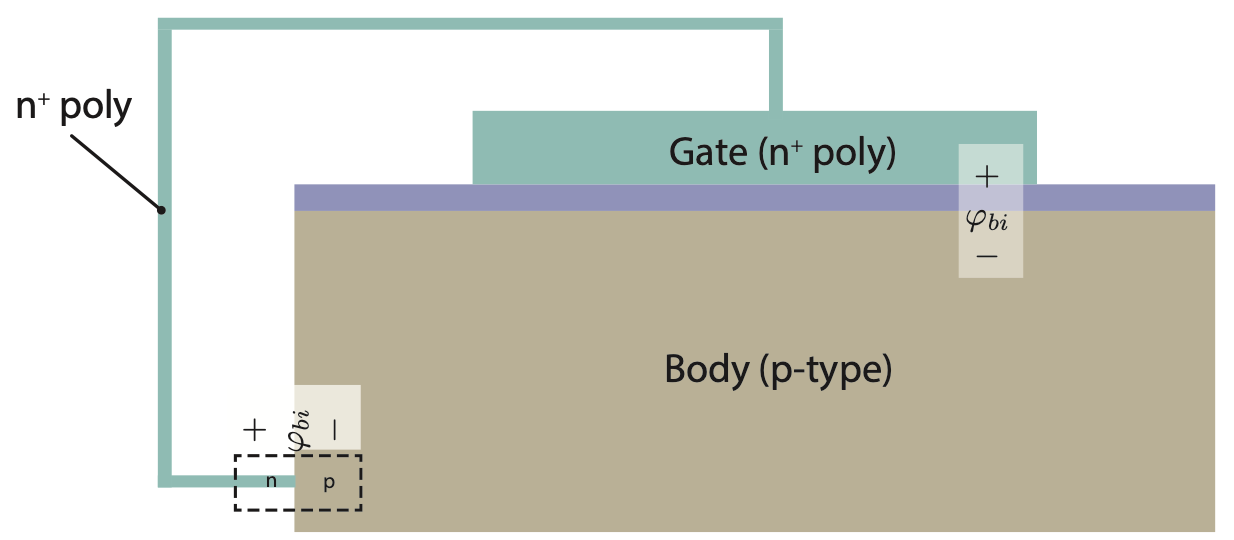
\includegraphics[scale=0.4]{figs/ch04/moscap_short2.png}
    \caption{There is a $\phi_{bi}$ from across the PN junction that leads to potential drop across the oxide}
\end{figure}

\begin{gline}
    \item[] Potential of the $P$ type region substrate: $\phi_p = -(\frac{kT}{q}) \ln(\frac{N_A}{n_i})$ 
    \item[] Potential of the $N$ type gate: $\phi_{poly,n+} = (\frac{kT}{q}) \ln(\frac{N_{d,poly}}{n_i})$
    \item[] Built in potential, NMOS Cap: $\phi_{bi} = \phi_{poly,n+} - \phi_p$
\end{gline}
In practice, real wires made of metal like aluminum or copper are used to connect the gate to the body. At the body side, this metal is connected to a heavily doped $p^+$ region. The \textbf{flatband voltage}, $V_{FB}$, is defined as the gate to body voltage that results in net zero charge and zero fields in the MOSCAP structure. The name comes from the observation that energy bands are flat whe the charge on the gate goes to zero and the depletion region disappears.
    \[V_{FB} = -\phi_{bi} = -(\phi_{n^+} - \phi_p)\]

Due to the difference in materials that make up the gate and body, we have an electric field from the gate to the body. 
\section{Regions of Operation}
There are three regions of operation: accumulation, depletion, and inversion. 

\subsection{Accumulation}
The MOSCAP operates under accumulation when $V_{GB} < V_{FB}$. $V_{GB}$ is the gate to body voltage. This looks like a parallel plate capacitor where there are many electrons and holes to charge up the plates. Negative charges/electrons can flow into the gate and holes will \textbf{accumulate} on the surface of the device. This is because negative bias attracts holes to reside under the gate. 

\subsection{Depletion}
The MOSCAP operates under depletion when $V_{GB} > V_{FB}$. An artificial depletion region is formed if you apply a voltage to the gate of the MOS CAP. When this happens we are in depletion mode. This is similar to the MOS CAP being in equilibrium.

\subsection{Inversion}
The MOSCAP operates under inversion when $V_{GB} = V_{FB}$.
\begin{todo}
    \item might be a good idea to expand on this
\end{todo}

\section{Practice Problems}

\section{Sources}
\begin{itemize}
    \item 
\end{itemize}

% MOSFET
\newpage 
\chapter{MOSFETs}
A transistor comes from the two words \textbf{trans}conductance res\textbf{istor}. MOSFET stands for MOS field effect transistor since we are taking the MOS CAP and adding two extra diffusion regions. Most of the EE105 reader spents time on the NMOS device since most of the concepts can be carried over into analyzing the PMOS device too. A MOSFET is a three terminal device, so we are moving on form the junction diode, a basic two terminal device

Part of the motivation for learning about MOSFETs is for building a current source and also for voltage amplification. If we are able to form a voltage controlled current source, we can build a voltage amplifier.

\section{Structure}
\begin{gline}
    \item $n^+$: heavily doped $n$-type silicon
    \item $n^-$: lightly doped $n$-type silicon
    \item $V_t$: threshold voltage
    \item $V_T$: thermal voltage
    \item $L$: channel length
\end{gline}

\begin{figure}[htb]
    \centering
    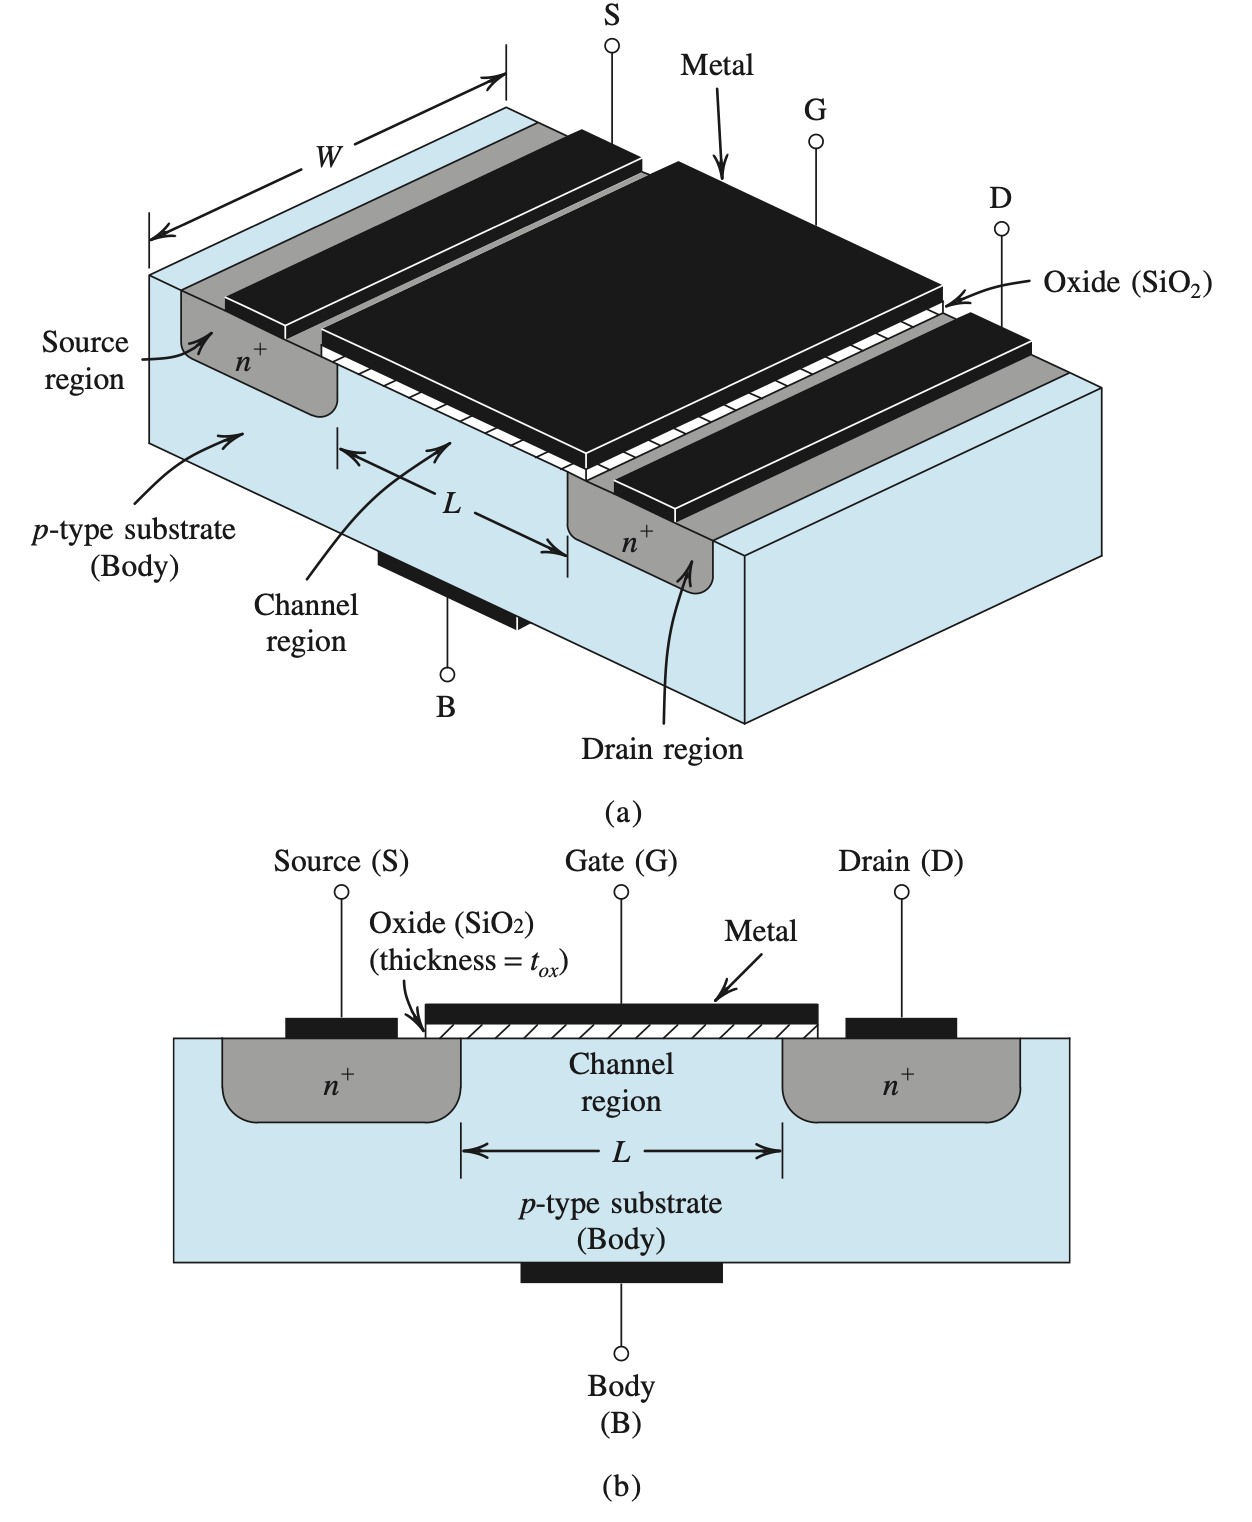
\includegraphics[scale=0.4]{figs/ch05/nmos_structure.png}
    \caption{Physical structure of the NMOS transistor and a cross section view}
    \label{fig:nmos_structure}
\end{figure}
In figure \ref{fig:nmos_structure}, we see that the NMOS transistor has the gate, source, drain, and substrate/body terminal, as indicated by the first letters of each terminal. From its physical structure, we notice that a MOSFET is a symmetrical device and that the substrate forms a PN junction with the source and drain regions.

At zero gate voltage, we see that there are two back to back diodes in series between drain and source. One from the PN junction formed between the $n^+$ drain region and the $p$ type substrate and the other from the $n^+$ source region and the $p$ type substrate. These diodes prevent current conduction from drain to source when a voltage $v_{ds}$ is applied.

\section{NMOS: Current conduction}
Suppose you ground the source and drain and $v_g > 0$. A positive gate voltage causes free holes to be repelled to the region of the substrate under the gate into the substrate. This leaves a \textbf{carrier-depletion region}. A positive gate voltage also attracts electrons from the $n^+$ source and drain regions to the channel region. Show in figure \ref{fig:nmos_conduct}
\begin{figure}[H]
    \centering
    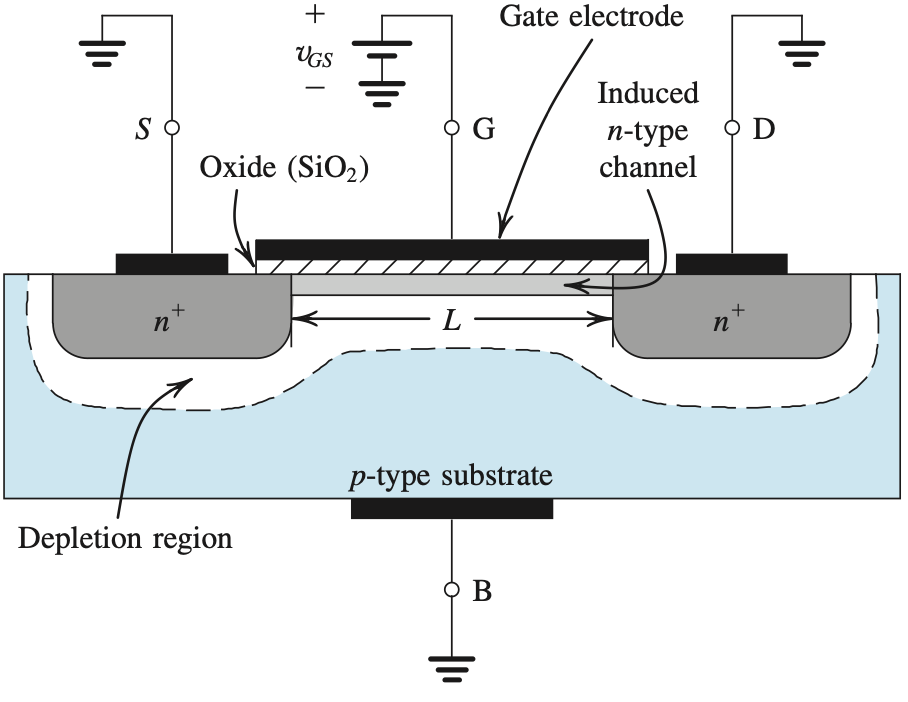
\includegraphics[scale=0.4]{figs/ch05/nmos_conduct}
    \caption{Positive voltage applied to the gate. An $n$ channel is induced at the top of the substrate beneath the gate}
    \label{fig:nmos_conduct}
\end{figure}
We see that a \textbf{channel} is formed for current flow from the drain to source. \textbf{Threshold voltage} is also defined as the value of \vgs where a sufficient number of mobile electrons accumulate in the channel region to form a conducting channel. \textbf{Overdrive voltage}, or \textbf{effective voltage} is the excess of \vgs over $V_t$. 
    \[v_{gs} - V_t \equiv v_{ov}\]
As \vov increases, so does the magnitude of the channel charge. If drawn out, this looks like the an increase in the depth/deepness of the channel.

Another thing to keep in mind here is the \textbf{oxide capacitance}.
    \[C_{ox} = \frac{\epsilon_{ox}}{t_{ox}}\]
\begin{gline}
    \item $C_{ox}$: capacitance of the parallel-plate capacitor per unit gate area, F/m\sq
    \item $\epsilon_{ox}$: permittivity of silicon dioxide; $\epsilon_{ox} = 3.9 \epsilon_0 = 3.45 \times 10^{-11}$ F/m
    \item $t_{ox}$: oxide thickness, determined by process technology
\end{gline}

\begin{Analysis}{Deriving $i_D$ for small \vds}{}
    We start by applying a small \vds and \vgs greater than its threshold voltage. $i_D$ is the current that Since $i_D$ is the charge per unit channel length, 
        \[\frac{\mid Q \mid}{\text{unit channel length}} = C_{ox} W v_{OV}\]
    We also know that channel conductance is proportional to the overdrive voltage, or \vgs $-V_t$. This means that current in the channel, $i_D$, is proportional to(\vgs $-V_t$). \vds also establishes an electric field $E$ across the length of the channel given by:
        \[\mid E \mid = \frac{v_{DS}}{L}\]
    An electric field causes channel electrons to drift towards the drain with a velocity of:
        \[\text{Electron drift velocity} = \mu_n \mid E \mid = \mu_n \frac{v_{DS}}{L}\] 
    Remembering that current is the rate of charged particles, then we find current by multiplying charge per unit channel length by the electron drift velocity.
        \[i_D = [(\mu_n C_{ox}) (\frac{W}{L}) v_{OV}] v_{DS} = [(\mu_n C_{ox}) (\frac{W}{L}) (v_{GS} - V_t)] v_{DS}\]
    Conductance of the channel is given by:
        \[g_{DS} = (\mu_n C_{ox}) (\frac{W}{L}) v_{OV} = (\mu_n C_{ox}) (\frac{W}{L}) (v_{GS} - V_t)\]
    \textbf{Process transconductance parameter} is given by:
        \[K_n' = \mu_n C_{ox}\]
\end{Analysis}

For a small \vds, the MOSFET behaves with a linear resistance $r_{DS}$ given by
    \[r_{DS} = \frac{1}{g_{DS}} = \frac{1}{(\mu_n C_{ox})(W/L)v_{OV}}\]

\begin{figure}[htb]
    \centering
    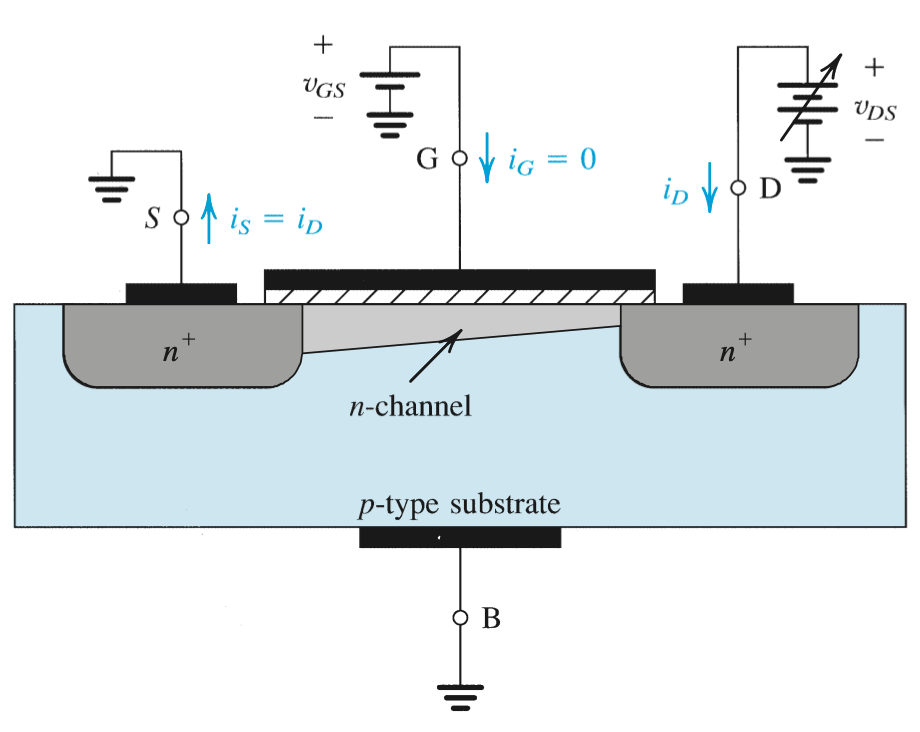
\includegraphics[scale=0.5]{figs/ch05/increase_vds.png}
    \caption{Operation of the enhancement NMOS transistor as \vds is increased}
    \label{fig:increase_vds}
\end{figure}

If we increase \vds, the depletion region will widen at the depletion region as a result of the increased \vds that makes the channel shallower near the drain. This is reflected in the formula for $i_D$. We'll see that the channel looks more like a tapered shape, where it's deepest at the source end (proportional to \vov) and shallowest at the drain end (proportional to \vov - \vds). Shown in figure \ref{fig:increase_vds}.
\[i_D = \mu_n C_{ox} (\frac{W}{L}) (V_{OV} - \frac{1}{2}v_{DS})v_{DS}\]

\begin{figure}[htb]
    \centering
    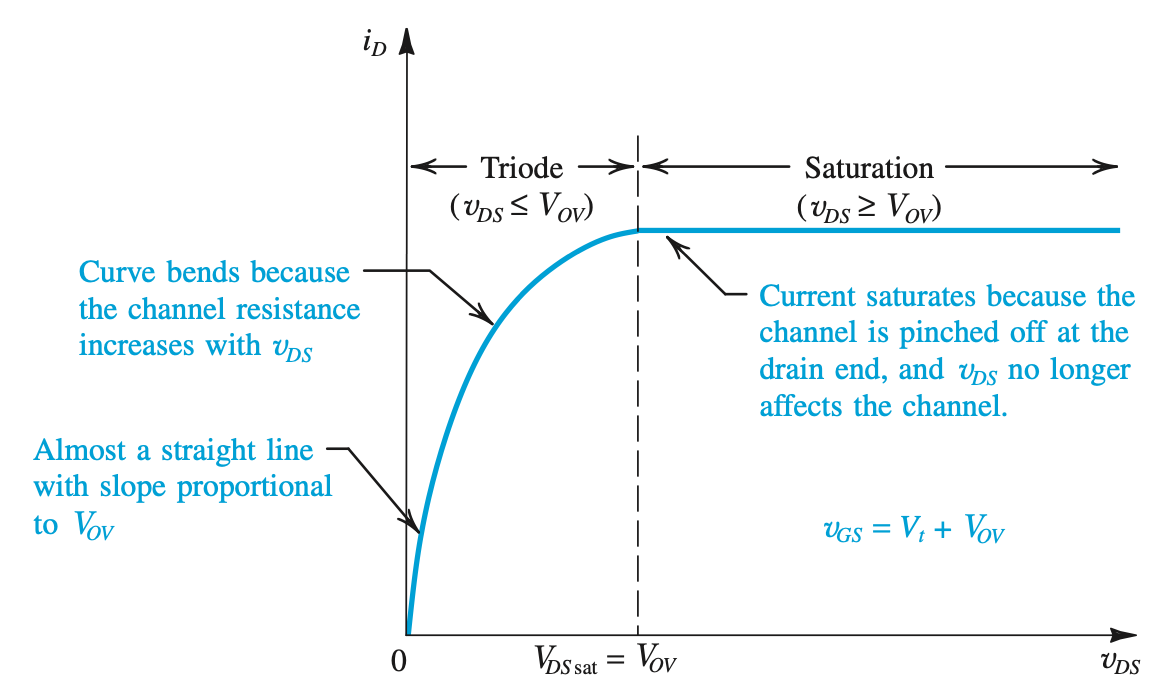
\includegraphics[scale=0.5]{figs/ch05/pinch_off.png}
    \caption{Operation of the enhancement NMOS transistor in different regions}
    \label{fig:pinch}
\end{figure}

Figure \ref{fig:pinch} shows the drain current for different regions. Increasing \vds beyond \vov has no affect on the channel shape and charge. This is when the transistor enters saturation and the channel region resembles a right triangle with the deepest part being close to the source.

\section{PMOS: Structure and Current conduction}
\begin{figure}[htb]
    \centering
    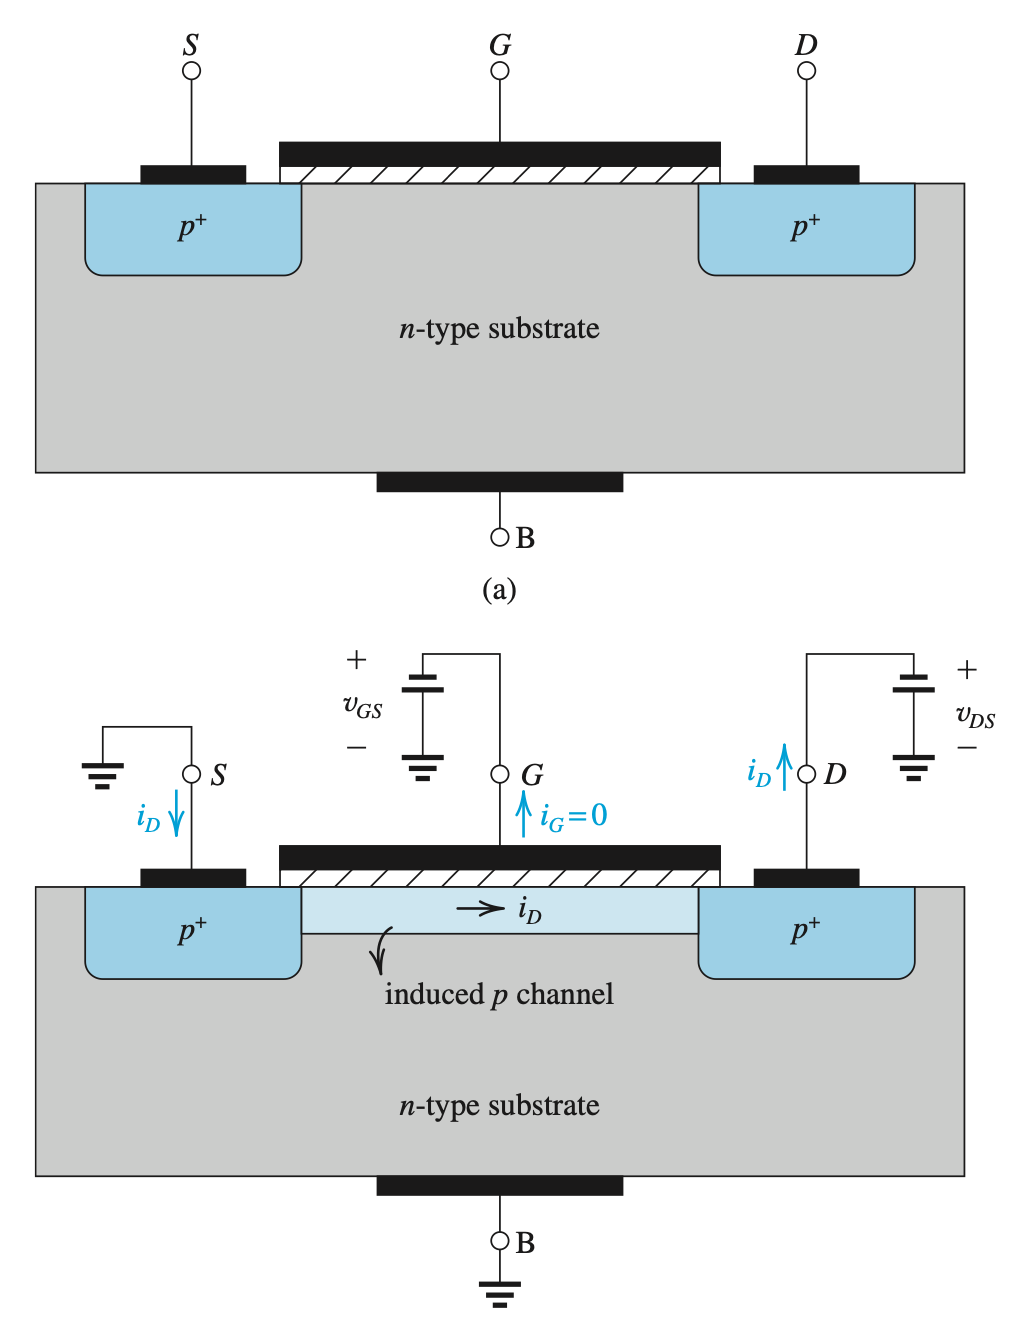
\includegraphics[scale=0.5]{figs/ch05/pmos_structure.png}
    \caption{Physical structure of the PMOS structure and side view}
    \label{fig:pmos_structure}
\end{figure}
To conduct current here, we need to apply a negative voltage between the gate and the source. This is because the current here is carried by holes (current goes in the same direction as the holes, contrastingly from when current is carried by electrons) and flows from the source to the drain. If we had to compare the NMOS cross section with the PMOS cross section, then we would notice that the substrate type for a PMOS transistor is an $n$-type substrate with $p^+$-type wells for the source and drain, while this is switched for a NMOS transistor ($p$-type substrate with $n^+$-type wells for source and drain). We'll also notice that the direction of current is flowing from opposite wells.
\begin{gline}
    \item $k'_p = \mu_p C_{ox}$: process transconductance parameter for PMOS
    \item $mu_p$: mobility of the holes in the induced 
    \item $k_p = k'_p(W/L)$: transistor transconductance parameter
\end{gline}

Typically, NMOS transistors have greater gain and speed of operations than PMOS devices. Electron mobility $\mu_n$ is higher by factor of 2 to 4 than the hole mobility $\mu_p$. The following attached PDF was something found online but sums up everything pretty nicely in a funny style.

\newpage %commenting this out for now so that its not so intensive to create test pdfs
% 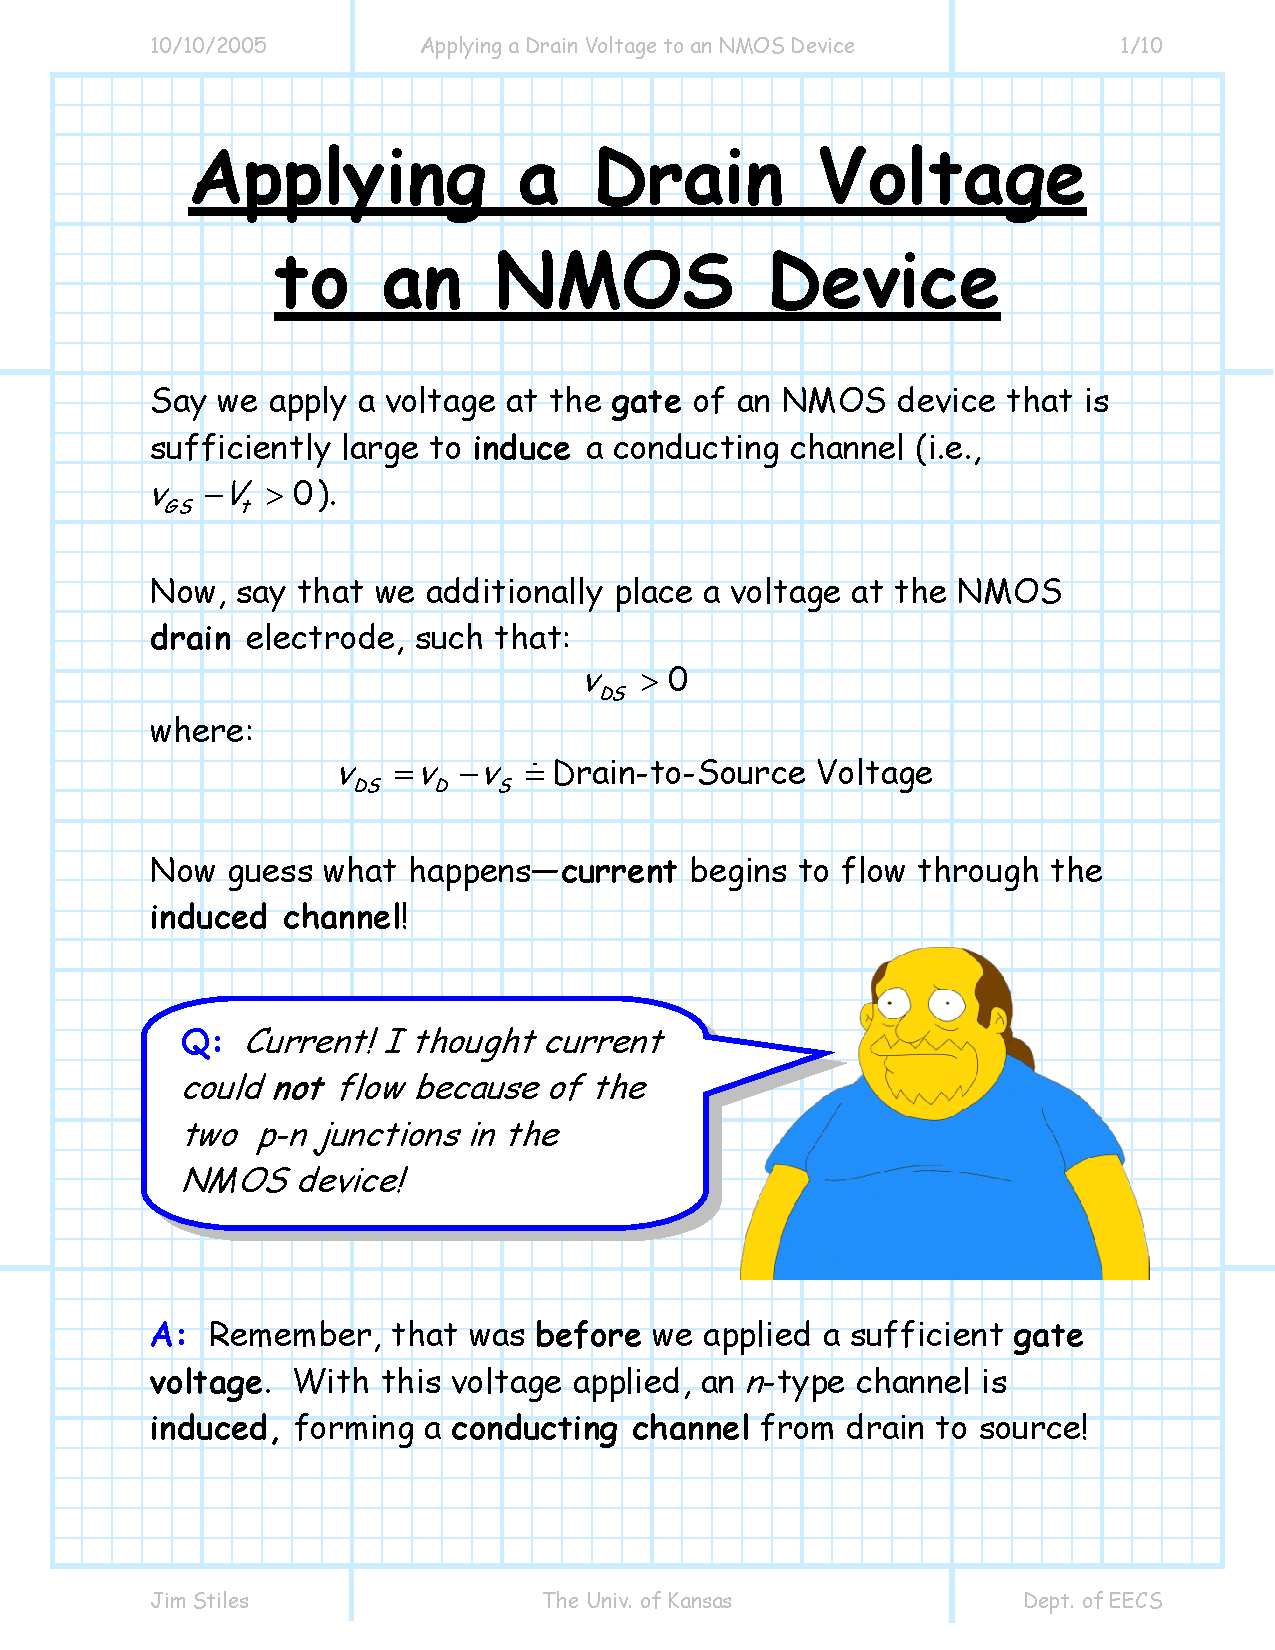
\includepdf[scale=0.9, clip, trim=10mm 10mm 10mm 10mm, pages={1-10}]{chapters/Applying_drain_voltage_nmos.pdf}


\section{Large and Small Signal Equivalent Models}
Large signal equivalent model of an $n$-channel MOSFET operating in the saturation region
\begin{figure}[H]
    \centering
    % \begin{circuitikz}[american voltages]
    %     \draw
    %       (0,0) to [short, o-] (6,0)
    %       to [V, l_=$\mathrm{j}{\omega}_m \underline{\psi}^s_R$] (6,2) 
    %       to [R, l_=$R_R$] (6,4) 
    %       to [short, i_=$\underline{i}^s_R$] (5,4) 
    %       (0,0) to [open, v^>=$\underline{u}^s_s$] (0,4) 
    %       to [short, *- ,i=$\underline{i}^s_s$] (1,4) 
    %       to [R, l=$R_s$] (3,4)
    %       to [L, l=$L_{\sigma}$] (5,4) 
    %       to [short, i_=$\underline{i}^s_M$] (5,3) 
    %       to [L, l_=$L_M$] (5,0); 
    % \end{circuitikz}
    \begin{circuitikz}[american voltages]
        \draw 
        (0,0) coordinate(a) 
            to [short, o-o] ++(10,0) 
        coordinate(b) 
            to (a) 
            to [open, -o] ++(0,2) coordinate(c)
            to [short,-o, i=$i_G$] ++(1,0)
            to [open, v=$v_{GS}$] ++(0,-2)
            to (b)
            to [open, v<=$v_{DS}$] ++(0,2) coordinate(d)
            to [short, i=$i_D$] ++(-1,0)
            to [short] ++(-6,0)
            to [cI, -*, l=$\frac{1}{2} k'_n \frac{W}{L}(v_{GS} - V_{tn})^2$] ++(0,-2)
            to ++(-1,0)
            to [short, *-o, l=S] ++(0,-0.5)
            to [open, -*] ++(6,0.5)
            to [R, -*, l_=$r_o$] ++(0,2)
            ;
    \end{circuitikz}
    \caption{Large signal model operating in saturation drawn with outputresistance $r_o$}
\end{figure}

\section{A More Complete Model}

\begin{figure}[H]
    \centering
    \begin{circuitikz}[scale=0.6, american voltages]
        \ctikzset{bipoles/resistor/height=0.15}
        \ctikzset{bipoles/resistor/width=0.4}
        \ctikzset{bipoles/capacitor/height=0.35}
        \ctikzset{bipoles/capacitor/width=0.1}
        \coordinate (G) at (0,0);
        \coordinate (D) at (14,0);
        \coordinate (S) at (0,-3);
        \coordinate (B) at (0,-6);
        \coordinate (curr1) at (4,0);
        \coordinate (curr2) at (7.75,0);
        \coordinate (res) at (11,0);
        \coordinate (Cdb) at (13,0);
        \draw 
        (G) 
            to [short, o-*] ++(1,0) node[label=left:G] at (G){}
            to [C, -*, l=$C_{gd}$] (curr1)
            to [short, -*] (curr2) 
            to [short, -*] (res)
            to [short, -*] (Cdb)
            to [short, -o] (D) node[label=right:D] {}
            to [open, i=$i_{ds}$] ++(-3,0)
        (G) 
            to [open] ++(1,0)
            to [C, -*, l=$C_{gs}$, v=$v_{gs}$] ++(0,-3)
            to [C, -*, l=$C_{sb}$, v<=$v_{bs}$] ++(0,-3)
        (S)
            to [short, o-*] ++(1,0) node[label=left:S] at (S){}
        (B)
            to [short, o-*] ++(1,0) node[label=left:B] at (B){}
            to ++(12,0)
        (curr1)
            to [cI, -*, l=$g_m v_{gs}$] ++(0,-3)
        (curr2)
            to [cI, -*, l=$g_{mb} v_{bs}$] ++(0,-3)
        (res)
            to [R, l=$r_o$] ++ (0,-3)
            to (S)
        (Cdb)
            to [C, l=$C_{db}$] ++(0,-3)
            to ++(0,-3)
            to (B)
        ;
    \end{circuitikz}
    \caption{A more complete NMOS model that is complete with capacitances.}
\end{figure}

With this model, we can rewrite \ids as the following:
    \[i_{DS} = g_m v_{gs} + g_{mb} v_{bs} + \frac{1}{r_o} v_{ds}\]
We see that the more complete model for the PMOS transistor is also really similar with some minor differences

\begin{figure}[H]
    \centering
    \begin{circuitikz}[scale=0.6, american voltages]
        \ctikzset{bipoles/resistor/height=0.15}
        \ctikzset{bipoles/resistor/width=0.4}
        \ctikzset{bipoles/capacitor/height=0.35}
        \ctikzset{bipoles/capacitor/width=0.1}
        \coordinate (S) at (0,0);
        \coordinate (D) at (15,-3);
        \coordinate (G) at (0,-3);
        \coordinate (B) at (0,-6);
        \coordinate (curr1) at (4,0);
        \coordinate (curr2) at (7.75,0);
        \coordinate (res) at (11,0);
        \coordinate (Cdb) at (13,-3);
        \draw 
        (G) 
            to [short, o-*] ++(1,0) node[label=left:G] at (G){}
            to [C, -*, l=$C_{gd}$] ++(3,0)
            to (D)
            to [short, -o] (D) node[label=right:D] {}
            to [open, i<=$i_{ds}$] ++(-3,0)
        (G) 
            to [open] ++(1,0)
            to [C, -*, l=$C_{gs}$, v<=$v_{sg}$] ++(0,3)
            % to [C, -*, l=$C_{sb}$, v<=$v_{bs}$] ++(0,3)
        (S)
            to [short, o-*] ++(1,0) node[label=left:S] at (S){}
            to (res)
        (B)
            to [short, o-*] ++(1,0) node[label=left:B] at (B){}
            to ++(12,0)
        (curr1)
            to [cI, *-*, l=$g_m v_{sg}$] ++(0,-3)
        (curr2)
            to [cI, *-*, l=$g_{mb} v_{sb}$] ++(0,-3)
        (res)
            to [R, -*, l=$r_o$] ++ (0,-3)
        (Cdb)
            to [C, *-, l=$C_{db}$] ++(0,-3)
            to (B)
            to ++(1,0)
            to [C] ++(0,3)
        ;
    \end{circuitikz}
    \caption{A more complete NMOS model that is complete with capacitances.}
\end{figure}

How does this more complete model affect the amplification effect?

Future chapters will talk about the BJT (bipolar junction transistor). 
\begin{pline}
    \item MOSFETs can be made smaller than BJTs
    \item MOSFET manufacturing process is relatively simpler and requires comparatively little powers
    \item MOSFETs generate less heat
    \item BJT better for current amplification circuits
    \item BJT low on-state voltage drop and low conduction loss
    \item BJT preferred in high power applications due to higher power handling; MOSFET preferred for low power applications
\end{pline}

\begin{todo}
    \item reorganize these items into a gline into the appropriate section
    \item $C_{gs}$: gate-source capacitance in saturation
    \item $C_{ov}$: MOSFET parasitic overlap capacitance
    \item $C_{gd}$: gate-drain capacitance in saturation
    \item $C_{sb}$: source body capacitance
    \item $C_{db}$: drain body capacitance
    \item also make tex model for mosfet with the body capacitances and a complete model (lec4/4/24)
\end{todo}
\section{Practice Problems}
\begin{enumerate}
    \item Find the region of operation for the following transistors. You may use $V_{tn} = 0.9$V and $\mid V_{tp} = 1$V. The operation condition of NMOS is also shown. PMOS is conducted by holes which is opposite to NMOS so the voltage polarity is different.
    \begin{figure}[H]
        \centering
        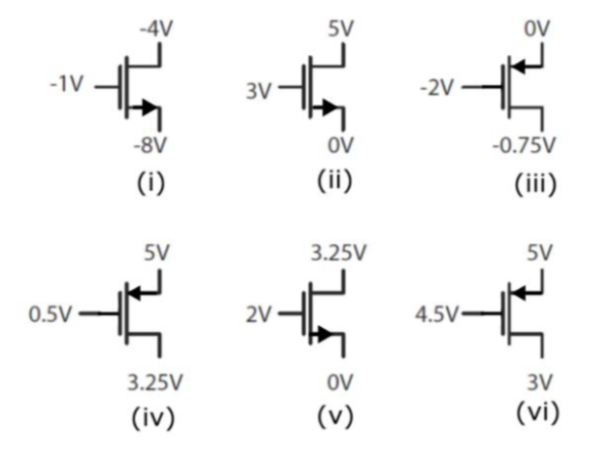
\includegraphics[scale=0.8]{figs/ch05/pp_transistor1.png}
    \end{figure}
    \begin{center}
        \begin{tabular}{|c|c|c|}
            \hline
            Region of operation & Condsitions & \ids \\
            \hline
            Cut-off & \vgs < $V_T$ & \ids $\sim$ 0A \\
            \hline
            Linear/Triode & $V_{GS}$ > $V_T$, $V_{DS} < V_{GS} - V_T$ & \ids = {\large $\frac{W}{L} \mu_n C_{ox} (V_{GS} - V_T - \frac{V_{DS}}{2}) V_{DS}$} \\ [10pt]
            \hline
            Saturation: & $V_{GS}$ > $V_T$, $V_{DS} > V_{GS} - V_T$ & {\large \ids = $\frac{W}{L} \frac{\mu_n C_{ox}}{2} (V_{GS} - V_T)^2 (1+ \lambda V_{DS})$} \\
            \hline
        \end{tabular}
    \end{center}
    \textcolor{blue}{
    \begin{enumerate}
        \item We identify this transistor as a NMOS transistor due to the direction of the arrow. In a NMOS transistor, current flows from drain to source due to electrons being the charge carriers in the NMOS transistor. \vgs = $v_G - v_S$ = 7V and \vds = $v_D - v_S = -4 -(-8) - 4$V. This transistor is in the linear/triode region. 
        \item \vgs = 3V and \vds = 5V. This transistor is in the saturation region.
        \item This is a PMOS transistor. In a PMOS transistor, current flows from source to drain. $|v_{GS}|= 2$V and $|v_{DS}|= 0.75$V. This is in the linear/triode region.
        \item $|v_{GS}| = 4.5$V and $|v_{DS}| = |3.25 - 5| = 1.75$V. This is in the linear/triode region.
        \item $v_{GS} = 2$V and $v_{DS} = 3.25-0 = 3.25$V. This is in the saturation region.
        \item $|v_{GS}| = |4.5-5| = 0.5$V. This is in the cutoff region.
    \end{enumerate}
    }

    \item An ideal $N$-channel MOSFET has the following parameters: $W = 100$ \mun, $L = 1$ \mun, $t_{ox} = 15$ nm, the oxide relative permittivity is 4, the silicon relative permittivity is 12, $N_A = 10^{15}$\conc, $n_i = 10^{10}$\conc, $V_{FB} = -0.2$ V, $\mu_n = 300$\mobility at 300K. $\lambda = 0$.
    \begin{enumerate}
        \item Find the threshold voltage.
        \begin{Ans}
            Threshold voltage is given by the following formula:
            \begin{align*}
                \phi_B &= \frac{kT}{q} \ln\frac{N_A}{n_i} = 0.026 V \ln(\frac{10^{15} \mathrm{ cm}^{-3}}{10^{10} \mathrm{ cm}^{-3}}) = 0.2993 \dots V \\
                C_{ox} &= \frac{\epsilon_{ox}}{t_{ox}} = \frac{4(8.854 \times 10^{-14} \mathrm{F/cm})}{15 \mathrm{nm}} = 3.54 \times 10^{-7} \mathrm{F/cm}^2 \\
                V_t &= V_{FB} + 2\phi_B + \frac{\sqrt{2q\epsilon_s N_A 2 \phi_B}}{C_{ox}} \\
                &= -0.2 + 2(0.299) + \frac{2(12)(8.854 \times 10^{14} \mathrm{F/cm})(1.602 \times 10^{-19} C)(10^{15} \mathrm{cm}^{-3})(2)(0.2993 V)}{3.54 \times 10^{-7} \mathrm{F/cm}^2} \\
                &= 0.44 \mathrm{V}
            \end{align*}
        \end{Ans}

        \item What is the minumum \vds value for the MOSFET to be at saturation region at \vgs = 2V. 
        \begin{Ans}
            For the MOSFET to remain in saturation, \vds = \vgs - $V_tn$, so 
            \[V_{DS} - V_{DS} - V_{tn} = 2 - 0.44 = 1.56 \mathrm{V}\]
        \end{Ans}

        \item Find the channel resistance at \vgs = 2V and \vds = 0.01 V.
        \begin{Ans}
            Channel resistance is given by calculating what \ids is given that we know \vds is. 
            \begin{align*}
                R_{ch} &= \frac{V_{DS}}{I_{DS}} = \frac{0.01 V}{\frac{W}{L} \mu_n C_{ox} (V_{GS} - V_T) V_{DS}} \\
                &= \frac{1}{300 \times 100 \times 3.54 \times 10^{-7} \times 1.56} \\
                &= 60.36 \Omega
            \end{align*}
        \end{Ans}

        \item Find $I_D$ at \vgs = 2V and \vds = 1V.
        \begin{Ans}
            At these values, the transistor is in the linear/triode region, so 
            \begin{align*}
                I_D &= \frac{\mu_n W}{L} C_{ox} ((v_{GS} - V_{tn}) v_{DS} - \frac{v_{DS}^2}{2}) \\ 
                &= 300 \times 100 \times 3.54 \times 10^{-7}(2 - 0.44) (1 - \frac{1^2}{2}) \\
                &= 0.011 A
            \end{align*}
        \end{Ans}        

        \item Find $I_D$ at \vgs = 2V and \vds = 2V.
        \begin{Ans}
            At these values, the transistor is in the saturation region.
            \begin{align*}
                I_D &= \frac{\mu_n W}{2 L} C_{ox} (v_{gs} - v_t)^2 \\
                &= \frac{300}{2} \times 100 \times 3.54 \times 10^{-7} \times (2-0.44)^2 \\
                &= 0.013 A
            \end{align*}
        \end{Ans}
    \end{enumerate}

    \item A circuit designer intending to operate a MOSFET in saturation is considering the effect of changing the device dimensions and operating voltages on the drain current $I_D$. Specifically, by what factor does $I_D$ change in each of the following cases?
    \begin{enumerate}
        \item The channel length is doubled.
        \begin{Ans}
            The problem says that the MOSFET is in saturation. $I_D$ in saturation is 
                \[I_D = \frac{1}{2} \mu_n C_{ox} (\frac{W}{L}) (v_{GS} - V_{tn})^2\]
            From the above equation, we see that $I_D$ is inversely proportional to channel length. So, if channel length is doubled then $I_D$ will be halved.
        \end{Ans}

        \item The channel width is doubled.
        \begin{Ans}
            $I_D$ will be doubled (refer to equation for $I_D$ in saturation above).
        \end{Ans}

        \item The overdrive voltage is doubled.
        \begin{Ans}
            Overdrive voltage is equal to \vgs - $V_t$, so $I_D$ will quadruple if the overdrive voltage is doubled.
        \end{Ans}

        \item The drain to source voltage is doubled.
        \begin{Ans}
            If we doubled \vds, there will be no effect on the drain current since \vds already reaches overdrive voltage drain current saturates and remains constant.
        \end{Ans}

        \item Changes (a), (b), (c), and (d) are made simultaneously.
        \begin{Ans}
            Simultaneously doing change (a) and change (b) results in the current remaining constant. Double the overdrive voltage results in drain current quadrupling while (d) will not change drain current so the drainc current will stay 
        \end{Ans}

        \item Which of these changes might cause the MOSFET to leave the saturation region?
        \begin{Ans}
            Decreasing \vds may cause this since this may change the channel underneath.
        \end{Ans}
    \end{enumerate}

    \item An $N$-channel MOSFET with the following parameters: $W = 10$\mun, $L = 1$\mun, $V_t  =0.5$V, $\mu_n = 400$ \mobility, \cox $=4\times10^{-7}$ F/cm\sq, $\lambda = 0.01 \mathrm{V}^{-1}$.
    
    \begin{figure}[H]
    \centering
    \begin{circuitikz}[american voltages]
        \ctikzset{tripoles/mos style/arrows}
        \coordinate (start) at (0,0);
        \draw 
        (start) node[nmos](nmos){} 
        (nmos.G) 
            to ++(-1,0) 
            to [sV, l_=$v_s$] ++(0,-1.5)
            to [V, l_=$V_{GS}$] ++(0,-1) node[ground]{}
        (nmos.S) 
            to ++(0,0) node[ground]{}
        (nmos.D) 
            to [short, *-o, l=$v_o$] ++(1,0)
        (nmos.D)
            to [R, *-*, l=$R_D$] ++(0,2)
            to ++(2,0)
            to [V, *-, v=$V_{DD}$] ++(0,-1.5) node[ground]{} 
        ;
    \end{circuitikz}
    \caption{Circuit for this problem}
\end{figure}

    \begin{enumerate}
        % STATIONARY WRAPFIGURE FORCED TO FLOAT: means that text paragraphs are too short to full wrap around the supplied figures
        \item Calculate \gm at \vgs = 1V and \vds = 1.2V.
        \begin{Ans}
            The formula is 
            \begin{align*}
                g_m &= \mu_n C_{ox} \frac{W}{L} (v_{GS} - V_t)(1 + \lambda V_{DS}) \\
                &=(400 \frac{cm^2}{V \cdot s})(4 \times 10^{-7} \frac{F}{cm^2})(\frac{10 \mu \mathrm{m}}{1 \mu \mathrm{m}})(1 V - 0.5V)(1+0.01 V^{-1} (1.2 V)) \\
                &= 8.096 \times 10^{-4} \Omega^{-1} \\
                &= 8.096 \times 10^{-4} S
            \end{align*}
        \end{Ans}

        \item Calculate $r_o$ at \vgs = 1V and \vds =1.2V.
        \begin{Ans}
            Formula for $r_o$ (output resistance) is 
            \begin{align*}
                r_o &= (\frac{\partial I_{DS}}{\partial v_{DS}})^{-1} \\
                &= \frac{1}{\mu_n C_{ox} \frac{W}{2L} (v_{GS} - V_t)^2  \lambda} \\
                &= \left( (\frac{400}{2} \frac{cm^2}{V \cdot s})(4 \times 10^{-7} \frac{F}{cm^2})(\frac{10 \mu \mathrm{m}}{1 \mu \mathrm{m}})(1 V - 0.5V) (0.01 V^{-1}) \right)^{-1} \\
                &= 500 k\Omega
            \end{align*}
        \end{Ans}

        \item Find the gain $\frac{v_o}{v_s}$ of this common source amplifier using this NMOS with \vgs = 1V, $R_D$ = 1 k$\Omega$ and \vdd = 1.4V. You can ignore the $\lambda$ when finding the DC bias point for simplicity. Don't need to consider capacitances and $g_{mb}$.
        \begin{Ans}
            Draw the small signal model.
            \begin{figure}[H]
    \centering
    \begin{circuitikz}[scale=0.6, american voltages]
        \coordinate (leftStart) at (0,0);
        \coordinate (rightStart) at (12,0);
        \draw 
        (leftStart)
            to [sV, l=$v_s$] ++(0,-4) node[ground]{}
            to [open, -*] ++(3,0) node[ground]{}
            to [open, -*, v<=$v_{GS}$] ++(0,4)
            to (leftStart) ++(-3,0)
        (rightStart)
            to [short, o-, l_=$v_o$] ++(-1,0)
            to [R, l=$R_D$] ++(0,-4)
            to ++(-2,0)
            to [R, l_=$r_o$] ++(0,4)
            to ++(-4,0)
            to [cI, l=$g_m v_{GS}$] ++(0,-4)
        (leftStart) 
            to [open] ++(5,0)
            to ++(7,0)
            to [open] ++(0,-4)
            to [short, o-] ++(-9,0)
        ;
    \end{circuitikz}
\end{figure}
            We see that \vgs = $v_s$. Find $v_o$ by Ohm's Law and equivalent resistance.
            \begin{align*}
                v_o &= -g_m v_{GS} (r_o || R_D) \\
                &= -g_m v_s (r_o || R_D) \\
                \frac{v_o}{v_s} &= -g_m (r_o || R_D) \\
                &= -8.096 \times 10^{-4} \Omega^{-1} (500 k\Omega || 1 k\Omega) \\
                &= -0.808
            \end{align*}
        \end{Ans}
    \end{enumerate}

    \item For a PMOS common source amplifier:
    \begin{figure}[H]
    \centering
    \begin{circuitikz}[american voltages]
        \ctikzset{tripoles/mos style/arrows}
        \coordinate (start) at (0,0);
        \draw 
        (start) node[pmos](pmos){} 
        (pmos.G) 
            to ++(-1,0) 
            to [sV, l_=$v_s$] ++(0,-1.5)
            to [V, l_=$V_{SG}$] ++(0,-1) node[ground]{}
        (pmos.D) 
            to [short, *-o, l=$v_o$] ++(1,0)
            to [open] ++(-1,0)
            to [R, *-, l=$R_D$] ++(0,-2) node[ground]{}
        (pmos.S)
            to ++(0,1)
            to ++(2,0)
            to [V, *-, v=$V_{DD}$] ++(0,-1.5) node[ground]{} 
        ;
    \end{circuitikz}
    \caption{Circuit for this problem}
\end{figure}

    \begin{enumerate}
        \item If $v_{SG} - |V_{tp}| = V_0$, and $k = \mu_p C_{ox} \frac{W}{L}$, find the maximum $R_D$ symbolically to make PMOS operation in the saturation region. Assume $\lambda = 0$. 
        \begin{Ans}
            For a PMOS transistor, it will be in saturation if $V_{SD} \geq V_{SD} - V_{tp}$
            \begin{align*}
                I_{DS} &= \frac{\mu C_{ox}}{2} \frac{W}{L} (V_{GS} - V_t)^2 \\ 
                &= \frac{k}{2} (V_{GS} - V_t)^2 \\
                &= \frac{k}{2} V_0^2 \\
                V_{SD} &= V_{DD} - R_D I_{DS} \geq V_0 \\
                V_{DD} - V_0 &\geq R_D I_{DS} \\
                V_{DD} - V_0 &\geq R_D \frac{k V_0^2}{2} \\
                R_D &\leq \frac{2 (V_{DD} - V_0)}{kV_0^2}
            \end{align*}
        \end{Ans}

        \item Draw its small-signal equivalent circuit and find out the $A_v = \frac{v_o}{v_s}$ symbolically ($R_D, g_m, r_o, g_{mb}$, and no capacitances). Please consider a finite PMOS output resistance ($r_o$) and assume it is in the saturation region. Body is grounded.
        \begin{Ans}
            \begin{figure}[H]
    \centering
    \begin{circuitikz}[scale=0.6, american voltages]
        \coordinate (leftStart) at (0,0);
        \coordinate (rightStart) at (12,0);
        \draw 
        (leftStart)
            to [sV, l=$v_s$] ++(0,-4) node[ground]{}
            to [open, -*] ++(3,0) node[ground]{}
            to [open, -*, v<=$v_{GS}$] ++(0,4)
            to (leftStart) ++(-3,0)
        (rightStart)
            to [short, o-, l_=$v_o$] ++(-1,0)
            to [R, l=$R_D$] ++(0,-4)
            to ++(-2,0)
            to [R, l_=$r_o$] ++(0,4)
            to ++(-4,0)
            to [cI, l=$g_m v_{GS}$] ++(0,-4)
        (leftStart) 
            to [open] ++(5,0)
            to ++(7,0)
            to [open] ++(0,-4)
            to [short, o-] ++(-9,0)
        ;
    \end{circuitikz}
\end{figure}
            Notice that the small signal model for a PMOS and NMOS transistor are the same here.
            \begin{align*}
                v_o &= -gm v_s (r_o || R_D) \\
                A_v = \frac{v_o}{v_s} &= -g_m (r_o || R_D) \\
                A_v = \frac{v_o}{v_s} &= -g_m \frac{r_o R_D}{r_o + R_D}
            \end{align*}
        \end{Ans}

        \item For the same circuit in part (b) but the body is connected to $v_o$, find $A_v$.
        \begin{Ans}
            \begin{figure}[H]
    \centering
    \scalebox{0.9}{
        \begin{circuitikz}[american voltages]
            \ctikzset{tripoles/mos style/arrows}
            \coordinate (start) at (0,0);
            \draw 
            (start) node[pmos, bulk](pmos){} 
            (pmos.G) 
                to ++(-1,0) 
                to [sV, l_=$v_s$] ++(0,-1.5)
                to [V, l_=$V_{SG}$] ++(0,-1) node[ground]{}
            (pmos.D) 
                to [short, *-o, l=$v_o$] ++(1,0)
                to [open] ++(-1,0)
                to [R, *-, l=$R_D$] ++(0,-2) node[ground]{}
            (pmos.S)
                to ++(0,1)
                to ++(2,0)
                to [V, *-, v=$V_{DD}$] ++(0,-1.5) node[ground]{} 
            (pmos.bulk)
                to ++(0,-1)
            ;
        \end{circuitikz}
        \begin{circuitikz}[scale=0.6, american voltages]
            \coordinate (leftStart) at (0,0);
            \coordinate (rightStart) at (14,0);
            \coordinate (curr1) at (5,0);
            \coordinate (curr2) at (9,0);
            \coordinate (res) at (13,0);
            \draw 
            (leftStart)
                to [sV, l=$v_s$] ++(0,-4) node[ground]{}
                to [open, -*] ++(3,0) node[ground]{}
                to [open, -*, v<=$v_{GS}$] ++(0,4)
                to (leftStart) ++(-3,0)
            (rightStart)
                to [short, o-, l_=$v_o$] ++(-1,0)
                to (curr1)
            (curr1)
                to [cI, l=$g_m v_{GS}$] ++(0,-4)
            (curr2)
                to [cI, l=$g_{mb} V_{BS}$] ++(0,-4)
            (res)
                to [R, l=$r_o || R_D$] ++(0,-4)
                to ++(-10,0)
            ;
        \end{circuitikz}
    }
    \caption{Circuit for this problem}
\end{figure}
            The figures above show the body connected to $v_o$ and the equivalent small signal model. By superposition, we that 
                \[v_o = -(g_m V_{GS} + g_{mb} V_{BS}) r_o || R_D\]
            The following shows steps. We keep in mind there at $V_{BS} = v_o$ here $V_{GS} = v_s$ here.
            \begin{align*}
                A_v = \frac{v_o}{v_s} &= - \frac{(g_m V_{GS} + g_{mb} V_{BS})}{v_s} r_o || R_D \\
                \frac{v_o}{v_s (r_o || R_D)} &= - \frac{(g_m v_s + g_{mb} v_o)}{v_s} = - g_m  - g_{mb} \frac{v_o}{v_s} \\
                A_v (\frac{1}{r_o || R_D} + g_{mb}) &= -gm \\
                A_v &= -\frac{g_m (r_o || R_D)}{1+ g_{mb} (r_o || R_D)}
            \end{align*}
        \end{Ans}
    \end{enumerate}

    \item The figure shows the equivalent circuit of an NMOS common-gate amplifier. The NMOS transistor has $g_m = 15$ mA/V and a large $r_o$ (can be modeled as open circuit). You can ignore body effect in this problem.

    \begin{figure}[H]
    \centering
    \begin{circuitikz}[american voltages]
        \ctikzset{tripoles/mos style/arrows}
        \ctikzset{bipoles/resistor/height=0.15}
        \ctikzset{bipoles/resistor/width=0.4}
        \ctikzset{bipoles/capacitor/height=0.2}
        \ctikzset{bipoles/capacitor/width=0.1}

        \coordinate (start) at (0,0);
        \draw 
        (start) node[nmos,xscale=-1](nmos){} 
        (nmos.G) node[ground]{}
        (nmos.S) 
            to [R, l=10 k$\Omega$] ++(0,-1.5) node[inputarrow, rotate=-90]{}
        (nmos.S)
            to [short,-o, l_=$v_i$] ++(-1,0)
        (nmos.D)
            to [R, l=5k$\Omega$] ++(0,1.5) node[inputarrow, rotate=90]{}
        (nmos.D)
            to [C, *-*, l=$\infty$] ++(1.5,0)
            to [R, l=2k$\Omega$] ++(0,-1.5) node[ground]{}
            to [open] ++(0,1.5)
            to [short, -o, l=$v_o$] ++(0.5,0);
    \end{circuitikz}
    \caption{Circuit for this problem}
\end{figure}
    
    \begin{enumerate}
        \item Draw the small signal AC model of the circuit using source transformation to convert $v_i$ into a current source $i_{in}$.
        \begin{Ans}
            \begin{figure}[H]
    \centering
    \begin{circuitikz}[american voltages]
        \ctikzset{tripoles/mos style/arrows}
        \coordinate (G) at (0,0);
        \coordinate (S) at (0,-1.5);
        \coordinate (V) at (7,1);
        \coordinate (5k) at (5,1);
        \coordinate (currS) at (1,1);
        \draw 
        (G) to [short, o-, l=$G$] ++(-1,0) node[ground]{}
        (G) to [open, v^=$V_{GS}$] (S)
        (S) 
            to [short, o-, l_=$S$] ++(1,0) % for labeling purposes
            to ++(3,0)
            to [open] ++(0,-1.5) node[ground]{}
            to [I, l=$i_{in}$] ++(0,1.5) 
        (V)
            to [short, *-, l_=$v_o$] ++(-1,0)
            to (currS)
            to [cI, -*, l=$g_m V_{GS}$] ++(0,-2.5)
            to [R, l=10k$\Omega$] ++(0,-1.5) node[ground]{}
        (V) to [R, l=2k$\Omega$] ++(0,-2) node[ground]{}
        (5k) to [R, l=5k$\Omega$] ++(0,-2) node[ground]{}
        ;
    \end{circuitikz}
    \caption{Circuit for this problem}
\end{figure}
        \end{Ans}

        \item Find the gain $\frac{v_o}{i_{in}}$ as a numerical answer.
        \begin{Ans}
            At the $v_s$ node, we see that 
                \[g_m V_{GS} = -g_m v_s\]
            So, we get by KCL that 
                \[i_{in} = g_m v_s + i_{10k} = g_m v_s + \frac{v_s}{10k}\]
            At the node $v_o$ also by KCL and Ohm's Law:
            \begin{align*}
                g_m V_{GS} + \frac{v_o}{5k} + \frac{v_o}{2k} &= 0 \\
                g_m v_s &= v_o (\frac{1}{5k} + \frac{1}{2k}) \\
                v_o &= \frac{g_m v_s}{5k || 2k} = 1428.56 g_m v_s \\
                \frac{v_o}{i_{in}} &= \frac{1428.56 g_m v_s}{v_s (g_m + \frac{1}{10k})} \\
                \frac{v_o}{i_{in}} &= 1419 \mathrm{V/A}
            \end{align*}
            In the second to last line we are given what $g_m$ is so we can get a numerical answer here.
        \end{Ans}

        \item What is the input resistance $Z_{in}$ as a numerical answer. Consider the source resistor in this computation.
        \begin{Ans}
            Perform KCL at node $v_s$, which will rename $V_x$ here.
            \begin{align*}
                \frac{V_x}{10k} &= i_{in} + g_m V_{GS} = i_{in} - g_m V_x \\
                V_x &= 10k(i_{in}) - 10k(g_m V_x) \\
                V_x (1 + 10k(g_m)) &= 10k(i_{in}) \\
                \frac{V_x}{i_{in}} &= \frac{10k}{1+10k(g_m)} = \frac{10k}{1+10k(0.15)} \\
                &= Z_{in} \\
                &= 6.6622 \Omega
            \end{align*}
        \end{Ans}
    \end{enumerate}
\end{enumerate}


\section{Sources}
\begin{itemize}
    \item copy patse the sources from earlier chapters
\end{itemize}

% MICROELECTRONICS: AMPLIFIERS AND SIGNALS
\newpage
\chapter{Single Stage Amplifiers}
From the \textit{Microelectronics} textbook here's a diagram on four amplifier types before going into single stage amplifiers.
\begin{figure}[H]
    \centering
    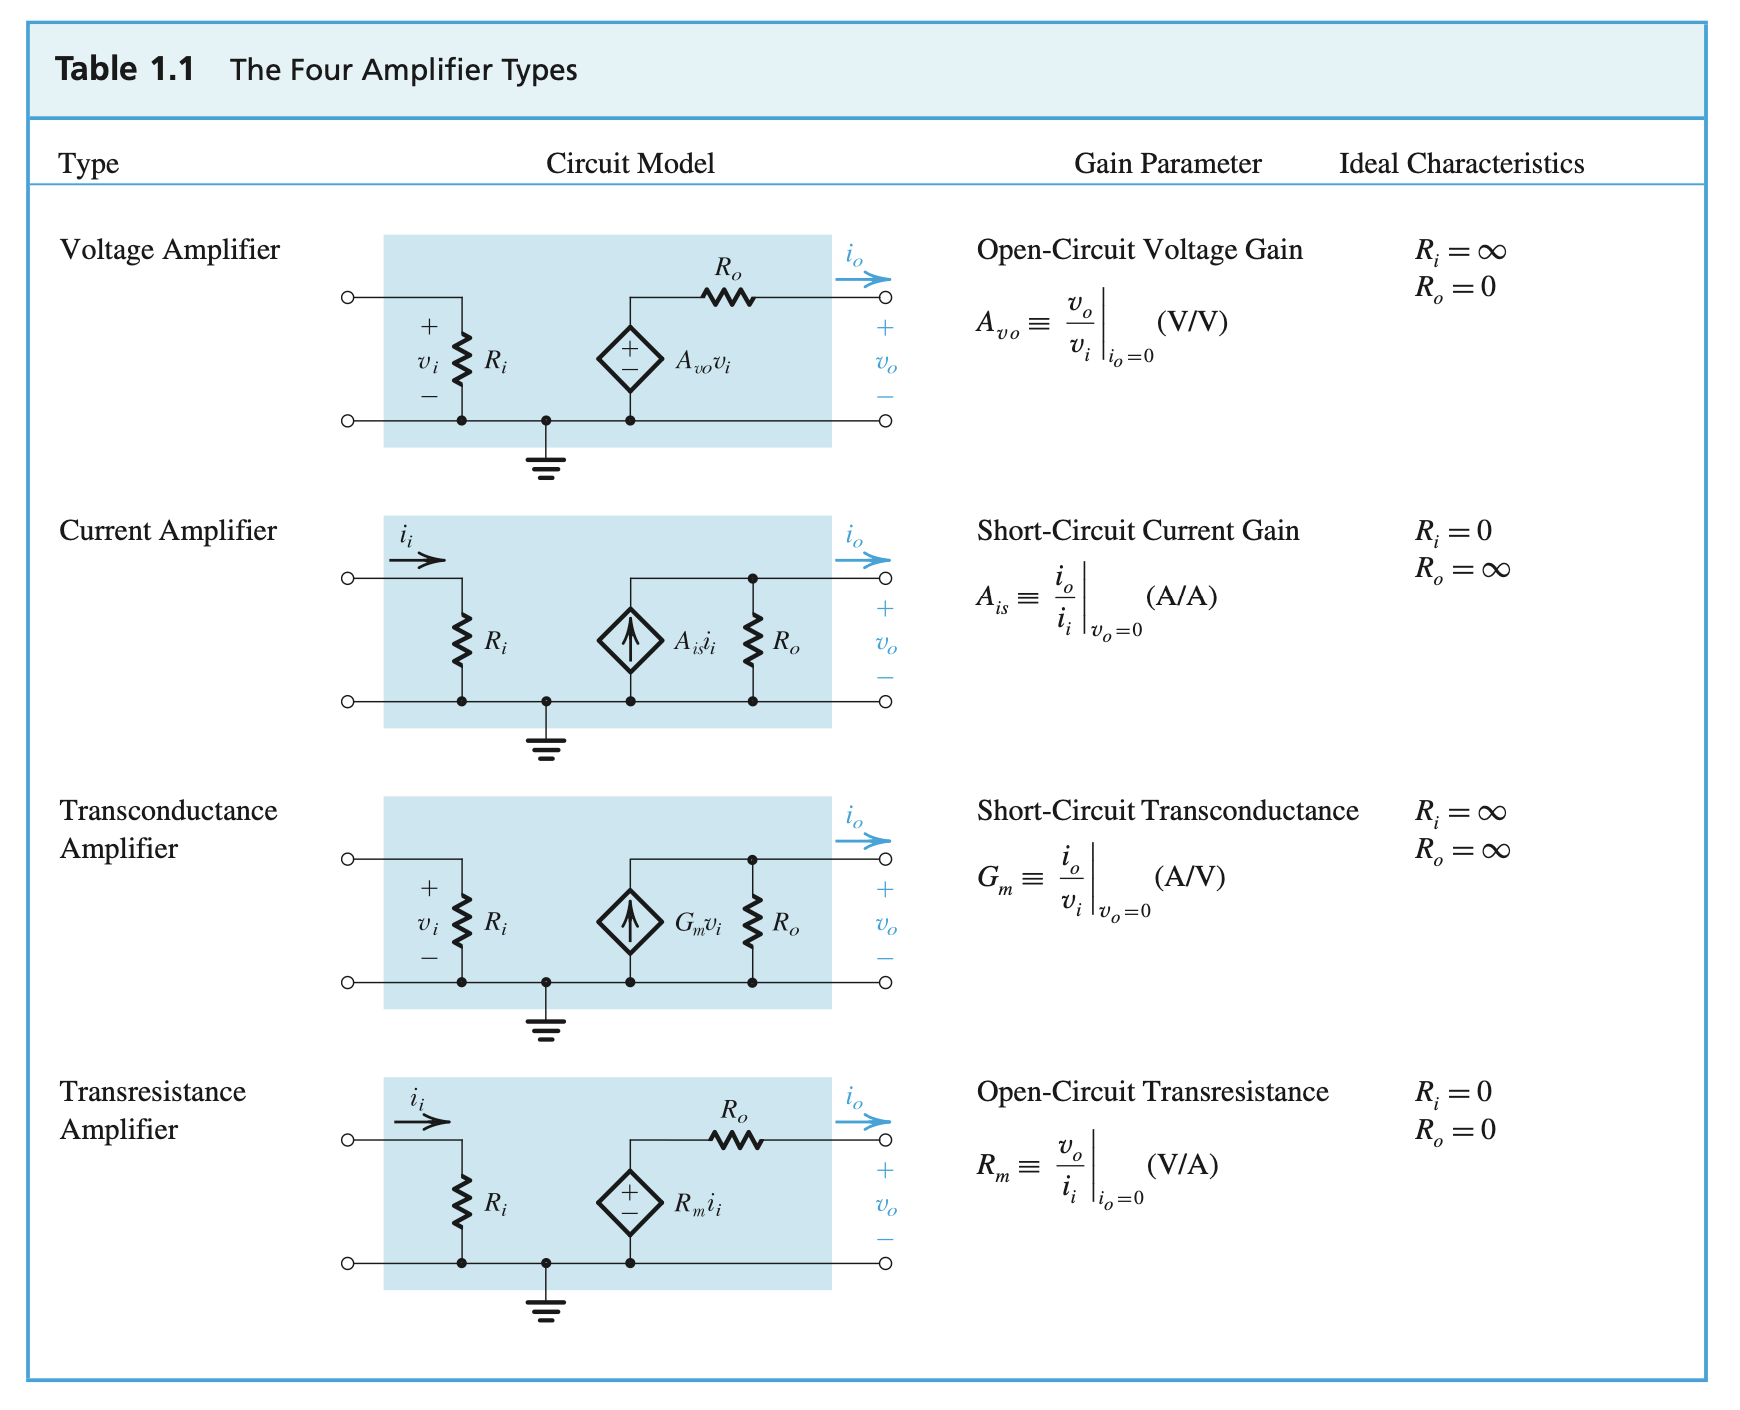
\includegraphics[scale=0.6]{figs/ch06/amplifier_types.png}
\end{figure}
In practice, there are other ways of finding input and output resistance, $R_i$ and $R_o$. You can find output resistance by measuring open-circuit output voltage to the short-circuit output current or by eliminating the input signal source and applying some voltage signal $v_x$ to the output of the amplifier. $R_o = v_x \slash i_x$. $i_x$ is the current frawn from $v_x$ into the output terminals. Input resistance can be found by measuring input current and input voltage.

If we ignore the body terminal of the MOSFET, we have a three terminal device. Since amplifiers is a four-terminal two-port, then this means that if we use two transistors one terminal must be common with each other. This leads to the following types of single stage amplifiers:
\begin{pline}
    \item Common source (CS) amplifier
    \item Common gate (CG) amplifier 
    \item Common drain (CD) amplifier
\end{pline}
BJT equivalents, respectively, are common emitter, common base, and common collector amplifiers. 

An inductor acts as an open circuit at high frequencies (remember by recalling its impedance, $j \omega L$ / $j 2 \pi f L$). We see that as we increase frequency, the impedance of the inductor increases as well. To summarize. an inductor at DC is a short-circuit and at AC is an open-circuit. The opposite is true for a capacitor. For this reason, infinitely large inductors, or \textbf{chokes}, are used in place of large resistors to isolate the \textit{DC supply or reference voltages} of sensitive circuits from the rest of the noisy system. 

AC coupling capacitors are ideally infinite and blocks DC, but allows AC to flow through.

\section{Common Source Amplifier}
Has the following parameters:
\begin{pline}
    \item Can develop gain
    \item High input impedance
    \item Inverting
\end{pline}

\section{Common Gate Amplifier}
A common gate amplifier has a current gain of unity, so it acts as a \textbf{currentÍ3‹ buffer}. It must meet the following requirements:
\begin{pline}
    \item Must have a current gain of unity
    \item Should present a low input impedance
    \item Should present a high output impedance
\end{pline}

\section{Common Drain Amplifier}
The signal input comes into the gate and the signal output leaves through the source and the drain is not grounded here and is instead connected to a DC voltage. Typically used as a \textbf{voltage buffer}.

\begin{todo}
    \item Insert into appropriate section
\end{todo}

\section{Practice Problems}

\begin{enumerate}
    \item Assume that the following circuits have the same large signal operating points and that $V_{tn}$ = 1V (without body bias), $k-n = \frac{\mu C_{ox} W}{L} = 10^{-3}$ A/V\sq, $\lambda = 0$, $\gamma = 0.5$ V$^{1/2}$, and $\phi_p = $ \SI{-400}{\milli \V}. $C_{big}$ means that the AC-coupling capacitor is so large that the lower bandwidth it imposes is far below any signal we are interested in and we can treat it as a short circuit for small-signal calculations (while still keeping it an open circuit for DC biasing calculations).
    \begin{todo}
        \item do this diagram is latex when you get the chance
    \end{todo}
    
    \begin{enumerate}
        \item What amplifier configurations are circuits
    \end{enumerate}
\end{enumerate}

\section{Sources}
\begin{itemize}
    \item EE105 Lecture 4/9/2024 by Alp Sipihigal
\end{itemize}
\end{document}